\documentclass[11pt]{article}
\usepackage[margin=1.15in]{geometry}
\usepackage{amsmath,amssymb,graphicx,xcolor,booktabs,needspace,placeins,xurl}
\usepackage[hidelinks]{hyperref}
\usepackage{listings}
\lstset{basicstyle=\ttfamily\small,breaklines=true,columns=fullflexible}
\newcommand{\E}{\mathbb E}
\newcommand{\Var}{\operatorname{Var}}
\emergencystretch=3em
\setlength{\parskip}{0.2em}
\renewcommand{\topfraction}{0.9}
\renewcommand{\bottomfraction}{0.8}
\renewcommand{\textfraction}{0.07}
\renewcommand{\floatpagefraction}{0.85}
\begin{document}
\begin{center}
{\LARGE Generating lensing maps on the DES footprint\par}
\vspace{0.6em}
{\large A student introduction to point-transformed Gaussian fields,\par}
{\large calibration from Rafael's maps, and covariance tests\par}
\vspace{0.5em}
22 November 2026
\end{center}

\section{What this experiment is trying to achieve}
\paragraph{Begin with a practical question.}
We have a finite collection of simulated shear maps supplied by Rafael
Gomes. We want to learn a much cheaper statistical generator from them,
then draw additional maps. The purpose is to test covariance estimation
for joint second- and third-order lensing measurements. Generating more
maps is useful only if their measured fluctuations are sufficiently
representative of the target. A generator that predicts the mean correctly
can still predict the covariance incorrectly.

\paragraph{The paper supplies a method, not our calibration.}
Zhong, Bernstein, Boruah, Jain and Kobla propose general point-transformed
Gaussian fields, abbreviated GPTG~\cite{zhong}. Their transformation is
more flexible than a lognormal mapping. They match one-point distributions
and angular two-point correlations, including correlations between source
bins. Their principal numerical tests use approximately seven-arcminute
pixels. The present implementation follows that construction but is our
own code and fit. It does not use an author-supplied four-bin calibration.
\textbf{We thank Kunhao Zhong and his coauthors for the method, Rafael Gomes
for the simulation maps, and the developers of ducc0 and HEALPix for the
spherical geometry and transforms.}

\paragraph{A route through this note.}
We first explain what a Gaussian field contains, then change its values
without randomly moving sky positions. Next we repair the power spectrum,
convert convergence into shear, apply the DES footprint and add a stated
noise model. Finally we describe the actual scripts and compare generated
measurements with the measurements used for calibration. Every approximation
in the first fit remains part of the interpretation of that comparison.

\paragraph{What an additional mock does and does not provide.}
A new random seed produces a new realization of the fitted stochastic
model. It supplies additional information about that model's covariance.
It does not create another independent gravitational N-body simulation.
Uncertainty in fitted parameters and shortcomings of the point transformation
remain even if we generate a million maps. This distinction determines
whether higher-order precision corrections are scientifically useful.

\section{From random numbers to a correlated sky}
\paragraph{One pixel is not yet a field.}
A standard Gaussian random number has mean zero and variance one. A
Gaussian field assigns such numbers to positions with specified correlations.
For two pixels, a simple example is
\begin{equation}
 g_1=u,\qquad g_2=\rho u+\sqrt{1-\rho^2}\,v,
\end{equation}
where $u$ and $v$ are independent standard Gaussian numbers. The first
variance is one. Expanding the second variance gives
\begin{equation}
 \E[g_2^2]=\rho^2\E[u^2]+2\rho\sqrt{1-\rho^2}\E[uv]
                 +(1-\rho^2)\E[v^2].
\end{equation}
Independence and zero means imply $\E[uv]=0$, while both squared means
are one. Therefore
\begin{equation}
 \E[g_2^2]=\rho^2+(1-\rho^2)=1.
\end{equation}
Their cross-correlation follows from one multiplication:
\begin{equation}
 \E[g_1g_2]=\rho\E[u^2]+\sqrt{1-\rho^2}\E[uv]=\rho.
\end{equation}
Independent pixels would set every nonzero-separation correlation to zero.
Such an image cannot test the covariance of a spatial lensing measurement.

\paragraph{Spherical harmonics organize correlations by angular scale.}
On the full sky, write a real field as a sum of spherical harmonics:
\begin{equation}
 g_i(\hat n)=\sum_{\ell=0}^{\ell_{\max}}
                   \sum_{m=-\ell}^{\ell} a^i_{\ell m}Y_{\ell m}(\hat n).
\end{equation}
The index $i$ labels a source-redshift bin. Small $\ell$ describes broad
angular variations; large $\ell$ describes finer structure. Statistical
isotropy specifies the covariance of the harmonic coefficients:
\begin{equation}
 \E[a^i_{\ell m}a^{j*}_{\ell' m'}]
       =C^{G,ij}_\ell\,\delta_{\ell\ell'}\delta_{mm'}.
\end{equation}
Different angular modes are independent in a Gaussian field, but the four
source bins can be correlated at each mode. Their four-by-four matrix
$C^G_\ell$ must be positive semidefinite: no combination of source fields
can have a negative variance.

\paragraph{Draw all source bins together.}
Factor the spectral matrix as
\begin{equation}
 C^G_\ell=A_\ell A_\ell^{\mathsf T}.
\end{equation}
An eigenvalue factorization allows zero eigenvalues; a Cholesky factor is
also possible when every eigenvalue is strictly positive. Draw a column
of four independent unit-variance Gaussian coefficients $z_{\ell m}$ and
multiply it by the factor:
\begin{equation}
 a_{\ell m}=A_\ell z_{\ell m}.
\end{equation}
Taking its covariance gives
\begin{equation}
 \E[a_{\ell m}a_{\ell m}^{\dagger}]
 =A_\ell\E[z_{\ell m}z_{\ell m}^{\dagger}]A_\ell^{\mathsf T}
 =A_\ell I A_\ell^{\mathsf T}=C^G_\ell.
\end{equation}
For $m>0$, real and imaginary parts each have half the variance. For
$m=0$, the coefficient is real and has the full variance. The negative
$m$ coefficients are fixed by the requirement of a real sky. Generating
each source bin independently would lose the desired cross-bin covariance.

\section{Changing the distribution while keeping the sky positions}
\paragraph{A local transformation is applied at every position.}
A point transformation takes a Gaussian value $g$ to a new value $f(g)$.
The same function is applied at every pixel within a source bin. It can
change skewness and tails, while the input correlations still connect
different positions. It does not reproduce every spatial dependence of
a nonlinear gravitational field; agreement must be tested on the statistics
we will actually measure.

\paragraph{Write the five-parameter function in two manageable pieces.}
Following Table 1 of Zhong et al., define the first factor
\begin{equation}
 h(g)=\exp(a_1g-a_1^2/2)+bg.
\end{equation}
The exponential gives a curved response; the linear term changes its
central shape and tail behavior. Define the transition factor separately:
\begin{equation}
 q(g)=\left[1+\exp\{t(g-x_0)\}\right]^{(a_2-a_1)/t}.
\end{equation}
The location $x_0$ places the transition and positive $t$ sets how rapidly
it occurs. The product before normalization is
\begin{equation}
 f(g)=h(g)q(g).
\end{equation}
Different parameters are allowed for different source bins.

\paragraph{Compute normalization from the ensemble distribution.}
For a standard Gaussian input, the mean is the integral
\begin{equation}
 \mu_f=\int_{-\infty}^{\infty}
       f(g)\frac{\exp(-g^2/2)}{\sqrt{2\pi}}\,dg.
\end{equation}
Subtracting this fixed mean centers the transformed field. Its variance is
\begin{equation}
 v_f=\int_{-\infty}^{\infty}
       [f(g)-\mu_f]^2\frac{\exp(-g^2/2)}{\sqrt{2\pi}}\,dg.
\end{equation}
Our code uses the unit-variance form
\begin{equation}
 F(g)=\frac{f(g)-\mu_f}{\sqrt{v_f}}.
\end{equation}
The physical convergence amplitude is then supplied by a separately stated
standard deviation $\sigma_\kappa$:
\begin{equation}
 \kappa=\sigma_\kappa F(g).
\end{equation}
This is a change of normalization of the paper's point-function family.
It lets the spectrum set the physical variance while the fit controls the
shape. The integrals use fixed Gauss--Hermite quadrature. We never subtract
each generated map's own mean or divide by its own measured variance: doing
so would remove random fluctuations whose covariance we want to estimate.

\paragraph{A good-looking central fit can still be invalid.}
The first trial fit to the downloaded maps produced a source-bin-two
function that turned over in a Gaussian tail. A central quantile fit alone
did not reveal that failure. To see the issue algebraically, first
differentiate the two factors:
\begin{equation}
 h'(g)=a_1\exp(a_1g-a_1^2/2)+b.
\end{equation}
The logarithmic derivative of the second factor is
\begin{equation}
 \frac{q'(g)}{q(g)}=(a_2-a_1)
                   \frac1{1+\exp[-t(g-x_0)]}.
\end{equation}
The product rule then gives
\begin{equation}
 \frac{f'(g)}{q(g)}=h'(g)+h(g)(a_2-a_1)
                   \frac1{1+\exp[-t(g-x_0)]}.
\end{equation}
The factor $q$ is positive, so the right-hand side determines the slope's
sign. We check it over the fitting region and Gaussian tails before drawing
maps. We retained the first failed attempt separately as debugging history;
it is not included in the subsequent pilot covariance.

\paragraph{A restricted family provides a transparent fallback.}
Setting $b=0$ recovers the paper's four-parameter double-log form. Its
logarithmic derivative simplifies to
\begin{equation}
 \frac{d\log f}{dg}=a_1+(a_2-a_1)s(g),
 \qquad s(g)=\frac1{1+\exp[-t(g-x_0)]}.
\end{equation}
Since $0<s<1$, rewrite the derivative as
\begin{equation}
 \frac{d\log f}{dg}=(1-s)a_1+s a_2.
\end{equation}
It is a weighted average of two positive numbers when $a_1,a_2>0$.
The function is then monotone for every real input. The current bin-two
fit uses this restriction and records it in its configuration. We do not
clip generated tail values to disguise a nonmonotone five-parameter fit.

\section{Why the Gaussian input spectrum must change}
\paragraph{A nonlinear map changes a correlation.}
Even if two Gaussian values have correlation $\rho$, their transformed
values generally do not. For centered unit-variance transformations, define
\begin{equation}
 H_{ij}(\rho)=\E[F_i(g_1)F_j(g_2)],
\end{equation}
where $(g_1,g_2)$ is jointly Gaussian with unit marginal variances and
correlation $\rho$. The desired convergence correlation is therefore
\begin{equation}
 \xi^{\kappa,ij}(\theta)=
 \sigma_{\kappa,i}\sigma_{\kappa,j}
 H_{ij}\!\left(\xi^{G,ij}(\theta)\right).
\end{equation}
The Gaussian correlation inside $H$ is dimensionless. The variance
factors outside restore the units and amplitudes of convergence.
Using the target convergence spectrum directly as the Gaussian input
would skip this nonlinear relation.

\paragraph{Invert one scalar relation at each angular separation.}
First divide the desired correlation by its two standard deviations:
\begin{equation}
 y_{ij}(\theta)=\frac{\xi^{\kappa,ij}(\theta)}
                         {\sigma_{\kappa,i}\sigma_{\kappa,j}}.
\end{equation}
Then solve for the Gaussian correlation:
\begin{equation}
 H_{ij}(\rho)=y_{ij}(\theta).
\end{equation}
The solution is the value to put into the Gaussian field at that
separation. A solution must lie between $-1$ and $1$. More strongly,
the complete set of solutions must produce positive semidefinite
spectral matrices for all multipoles. Valid pairwise correlations alone
do not prove that a multibin random sky exists.

\paragraph{Hermite functions make the correlation integral reusable.}
Let $\phi_n(g)$ be normalized probabilists' Hermite polynomials, with
$\phi_0=1$ and $\phi_1=g$. They are orthonormal under a unit Gaussian:
\begin{equation}
 \E[\phi_n(g)\phi_m(g)]=\delta_{nm}.
\end{equation}
Expand each centered transform in this basis:
\begin{equation}
 F_i(g)=\sum_{n=1}^{\infty}a_{in}\phi_n(g).
\end{equation}
Multiplying by $\phi_m$ and averaging isolates its coefficient:
\begin{equation}
 a_{im}=\E[F_i(g)\phi_m(g)].
\end{equation}
For correlated Gaussian inputs, the corresponding identity is
\begin{equation}
 \E[\phi_n(g_1)\phi_m(g_2)]=\delta_{nm}\rho^n.
\end{equation}
Insert both series into the desired two-point expectation before
simplifying the double sum:
\begin{equation}
 H_{ij}(\rho)=\sum_{n,m}a_{in}a_{jm}\delta_{nm}\rho^n.
\end{equation}
Only terms with equal indices survive, leaving
\begin{equation}
 H_{ij}(\rho)=\sum_{n=1}^{\infty}a_{in}a_{jn}\rho^n.
\end{equation}
The code evaluates coefficients once per fitted model, truncates at a
stated degree and tabulates this relation for inversion. Increasing the
Hermite degree and quadrature density is a numerical convergence test;
it does not add new physical information to the fitted model.

\paragraph{Connect angular correlations and spectra.}
For isotropic scalar fields, the correlation follows from the Legendre sum
\begin{equation}
 \xi^{ij}(\theta)=\sum_{\ell=0}^{\ell_{\max}}
       \frac{2\ell+1}{4\pi}C^{ij}_\ell P_\ell(\cos\theta).
\end{equation}
After the point-correlation inversion, transform back using
\begin{equation}
 C^{G,ij}_\ell=2\pi\int_{-1}^{1}
      \xi^{G,ij}(\arccos\mu)P_\ell(\mu)\,d\mu.
\end{equation}
The prototype uses fixed Gauss--Legendre nodes. Spectral interpolation,
finite multipole range and positivity repairs can disturb the requested
correlation. Their sizes must be reported, and generated spectra must be
measured again. Matching a table before those operations is not sufficient.

\section{Convergence becomes shear before the footprint is selected}
\paragraph{Shear is a spin-two field.}
A rotation of the local coordinate axes changes the two shear components.
A scalar point transform applied independently to those components would
not be the lensing construction in the paper. We transform convergence,
then obtain its two-component shear through spherical harmonics.
For multipoles $\ell\geq2$, the chosen convention relates them by
\begin{equation}
 \gamma^E_{\ell m}=
 -\sqrt{\frac{(\ell+2)(\ell-1)}{\ell(\ell+1)}}\,
 \kappa_{\ell m}.
\end{equation}
The minus sign is tied to the convention for the spin-harmonic basis.
The gravitational field in this pilot has no input B-mode. Monopole and
dipole convergence coefficients have no shear counterpart here.
The generated component basis must be checked against the basis of the
supplied maps before interpreting sign-sensitive third moments.

\paragraph{Why we generate a full sky.}
A full sky supplies correlated modes inside and outside the observed
region. A mask then selects the observed pixels. Generating only a
rectangular image and identifying it with DES would change the window,
long modes and boundary effects. The current implementation generates
NSIDE 512 skies and uses the exact supplied footprint list. The pilot
retains multipoles through 1024; this is a numerical choice to be tested,
not a claim that all observable contributions above it vanish.

\paragraph{The list of pixel IDs defines the saved array.}
There are
\begin{equation}
 N_{\rm full}=12(512)^2=3145728
\end{equation}
full-sky HEALPix pixels. The supplied list retains 369,190 of them.
For the saved shear array, the index relation is
\begin{equation}
 \texttt{map}[i,c,j]=\gamma_c^i(\texttt{indices}[j]).
\end{equation}
Here $i$ is the source bin and $c$ is the shear component. The last
axis is not a rectangular image axis. Reordering pixel IDs without the
same reordering of the map values changes the sky. We use the RING ordering
identified geometrically in the earlier footprint study.

\section{Adding and testing a shape-noise model}
\paragraph{State the first model explicitly.}
For each retained pixel, component and source bin, draw a zero-mean
Gaussian noise value independently. The observed synthetic shear is
\begin{equation}
 \gamma^{i,\rm obs}_c(p)=\gamma^{i,\rm signal}_c(p)+n^i_c(p).
\end{equation}
The assumed noise covariance is
\begin{equation}
 \E[n^i_c(p)n^j_d(q)]=\sigma_{n,i}^2\,
                \delta_{ij}\delta_{cd}\delta_{pq}.
\end{equation}
This initial model has constant noise variance within each source bin.
A DES catalogue can have position-dependent weights, number counts and
non-Gaussian ellipticities. Those are additional inputs or model tests;
constant independent Gaussian noise does not encode them automatically.

\paragraph{Where a variance estimate comes from.}
If one shear component of a galaxy has dispersion $\sigma_e$ and a pixel
contains $N_g$ equally weighted independent galaxies, averaging their
shapes gives
\begin{equation}
 \Var(n_c)=\frac1{N_g^2}\sum_{a=1}^{N_g}\sigma_e^2
          =\frac{\sigma_e^2}{N_g}.
\end{equation}
Writing the count as density times pixel area gives
\begin{equation}
 \sigma_{n}^2=\frac{\sigma_e^2}{n_g\Omega_{\rm pix}}.
\end{equation}
Here $\sigma_e$ is explicitly a \emph{per-component} dispersion; using a
two-component dispersion would require the corresponding factor of two.
Weighted catalogues replace the simple count by an effective count.

\paragraph{Our downloaded files do not supply that catalogue description.}
The first calibration estimates a constant noise level from high-multipole
masked B power, dividing by the sky fraction and equal pixel area. For a
pure white noise field this relation is motivated by
\begin{equation}
 N_\ell=\Omega_{\rm pix}\sigma_n^2.
\end{equation}
Multiplication by a footprint changes harmonic modes and creates E/B
leakage. Consequently our B-based estimate can include leaked signal;
it is an initial approximation, not an identification of the archive's
true noise-generation prescription. The generated E and B spectra and
aperture-noise statistics must expose whether it is sufficient.

\paragraph{Noise enters cubic measurements even when its mean is zero.}
Let one filtered aperture value be $A=s+n$, where $s$ is fixed and
$n$ is zero-mean Gaussian with variance $v$. Expand its cube:
\begin{equation}
 A^3=s^3+3s^2n+3sn^2+n^3.
\end{equation}
Average each term over noise:
\begin{equation}
 \E[A^3\mid s]=s^3+3s^2\E[n]+3s\E[n^2]+\E[n^3].
\end{equation}
The first and third noise moments vanish, while the second equals $v$:
\begin{equation}
 \E[A^3\mid s]=s^3+3sv.
\end{equation}
For a known, signal-independent $v$, the statistic $A^3-3vA$ has mean
$s^3$. Our raw-aperture comparison instead retains the same self-products
in both the downloaded and generated maps, matching the earlier diagnostic.
A published catalogue estimator can exclude repeated galaxies or apply
different corrections. Its formula must be matched separately.

\section{What the first calibration actually fits}
\paragraph{Choose a bounded and identifiable file selection.}
The first fit uses 32 run labels, always cut zero and realization zero.
The precise source filenames are recorded. This avoids silently counting
all realization labels as independent skies, whose production relationship
is still unresolved. It does not establish that the 32 selected runs are
statistically independent; it states the convention used by this pilot.

\paragraph{Measure both E and B pseudo-spectra.}
We insert the observed shear values into a zero-padded full-sky array and
apply the adjoint spin transform with equal-area pixel weights. In this
operation zero means a known missing-data window, not an observed galaxy
with zero shear. The resulting spectra are called pseudo-spectra because
the mask mixes angular modes. The initial signal estimate subtracts B
power from E power and divides by the sky fraction. We average within
multipole bands before interpolating. Exact mode-coupling deconvolution
is not part of this first fit.

\paragraph{Fit a distribution that can be measured with the available maps.}
The files contain shear, whereas the point transform is a model for
convergence. We reconstruct a filtered E-mode convergence proxy with the
same masked transform, smooth it at ten arcminutes, and evaluate it at
64 preselected interior positions. Quantiles of this reconstructed field
supply an initial point-function fit. They are not the distribution of
an unmasked, noiseless convergence sky. A subsequent forward comparison
must run generated maps through the same mask, reconstruction and filter.
Even a good comparison would constrain this measured proxy rather than
uniquely recover all underlying physical ingredients.

\paragraph{Why quantiles provide a simple fitting language.}
The $q$ quantile is the value below which fraction $q$ of the sample lies.
For a monotone function $F$, transforming a Gaussian quantile transforms
the corresponding output quantile:
\begin{equation}
 Q_F(q)=F\bigl(\Phi^{-1}(q)\bigr).
\end{equation}
Here $\Phi$ is the standard Gaussian cumulative distribution. The fit
uses probabilities from 0.02 to 0.98 and compares these predicted values
with measured standardized quantiles. A small residual over this interval
does not constrain extreme tails, nor does it establish that higher
moments or spatial correlations are correct. Boundary-hitting parameters
also signal that the data may not identify the chosen functional freedom.

\paragraph{Record repairs instead of presenting them as exact matching.}
Noisy cross-spectrum estimates can have negative eigenvalues. A covariance
for Gaussian harmonic draws cannot. The first pilot projects negative
eigenvalues to zero and records the fractional matrix change. After the
nonlinear correlation inversion it checks positivity again and normalizes
the latent Gaussian variances. Every such operation changes the requested
spectra. A later fit should improve the model or estimates when those
changes matter for measured observables; the code must not silently claim
exact spectrum matching after a repair.

\section{Programs, files and commands}
\paragraph{Use an activated Cocoa Python environment.}
The scripts require NumPy, SciPy, PyYAML and Astropy, already part of the
working scientific environment. The additional spherical-transform package
used in this test is ducc0 0.42.0. Install it with
\begin{lstlisting}
python -m pip install ducc0==0.42.0
\end{lstlisting}
The existing footprint and aperture reader additionally uses
astropy-healpix 1.0.3:
\begin{lstlisting}
python -m pip install astropy-healpix==1.0.3
\end{lstlisting}
Our tests installed these in temporary dependency directories instead of
modifying the shared Cocoa environment. Ordinary users can install them
in their selected environment. No separate Kunhao executable is downloaded:
\texttt{generate\_maps.py} is our documented implementation of the paper's
method. No CAMB call or N-body evolution is hidden inside it.

\paragraph{Keep the worker budget explicit.}
BLAS uses one worker. The transform worker count is set independently by
the script's command-line option, with a current maximum of eight. The ducc0
transforms use their native thread pool; setting a BLAS count does not
control that pool. The pilot used four workers. The later large run was authorized to use
eight; respect the current limit when reproducing a run. We generate maps serially so separate maps
do not each start their own four-worker computation concurrently.

\paragraph{Fit the initial model.}
From the activated Cocoa directory, run one command:
\begin{lstlisting}
python projects/des_3pcf/scripts/generate_maps.py fit --runs 32 --workers 4
\end{lstlisting}
This reads the listed original maps and writes fitted parameters and
small measurement records under \texttt{chains/gptg\_method/}. The originals
are unchanged. The YAML record gives source filenames, the harmonic cutoff,
noise amplitudes, point parameters and positivity-repair sizes.

\paragraph{Draw and save the new maps.}
The next command uses that saved fit:
\begin{lstlisting}
python projects/des_3pcf/scripts/generate_maps.py generate --count 64 --workers 4
\end{lstlisting}
The historical pilot used float64; recreating that precision reference
requires the explicit \texttt{--float64-reference} option in a fresh
output destination. The default for new maps is float32.
Each output has the same array shape and footprint ordering as a supplied
map. Names begin \texttt{GPTG\_DES\_} so the generated files cannot be
mistaken for Rafael's original realizations. The starting seed is recorded;
map number $r$ uses the starting seed plus $r$. Existing generated files
are not overwritten by another experiment. Preserve or move the old
experiment before deliberately rerunning the same output destination.

\paragraph{Measure the same quantities in both ensembles.}
The generator reuses the existing fixed aperture weights: 64 enclosed
centers, Gaussian shear filters at 30 and 60 arcminutes, and four source
bins. For each realization it averages squared and cubed aperture values,
producing sixteen raw moments. Thus the comparison includes third-order
measurements, but these coarse moments are not the published finite-triangle
three-point estimator. In the companion notebook, inspect the forward comparison and
tomographic noise-subtraction functions, then call them explicitly:
\begin{lstlisting}
compare_maps()
\end{lstlisting}
\begin{lstlisting}
measure_apertures()
\end{lstlisting}
The companion notebook shows the definitions,
normalizations and saved vectors before constructing their covariances.

\section{Measuring second and third moments, one operation at a time}
\paragraph{Start with one weighted aperture.}
The filter turns many shear pixels into one number at a chosen center.
Let $w_{1p}$ and $w_{2p}$ include pixel area, radial filter and the rotation
into tangential shear. For source bin $i$, the measured aperture is
\begin{equation}
 A_i=\sum_p\left(w_{1p}\gamma^i_1(p)+w_{2p}\gamma^i_2(p)\right).
\end{equation}
These weights are fixed by geometry. They do not depend on a map's measured
values. Write the aperture as signal plus filtered noise:
\begin{equation}
 A_i=s_i+\epsilon_i.
\end{equation}
For independent pixel components with the fitted variance, expand the
variance of the weighted noise sum. Cross terms between distinct pixels
or components vanish. What remains is
\begin{equation}
 v_i=\E[\epsilon_i^2]
 =\sigma_{n,i}^2\sum_p\left(w_{1p}^2+w_{2p}^2\right).
\end{equation}
The code uses the actual weights for each center. Even constant pixel noise
need not give exactly equal aperture noise at every center.

\paragraph{Correct the square before averaging over centers.}
Multiplying the two factors gives
\begin{equation}
 A_i^2=s_i^2+2s_i\epsilon_i+\epsilon_i^2.
\end{equation}
The signal is fixed while we average over added noise, so
\begin{equation}
 \E[A_i^2\mid s_i]=s_i^2+2s_i\E[\epsilon_i]+\E[\epsilon_i^2].
\end{equation}
The zero mean removes the middle term; the last term is $v_i$. Subtracting
that known contribution gives a statistic with the desired conditional mean:
\begin{equation}
 \E[A_i^2-v_i\mid s_i]=s_i^2.
\end{equation}
This is a correction to an aperture measurement. It is different from the
Wishart noisy-matrix-square correction in the precision-expansion note.
Both involve a noisy square, but they act on different random quantities.

\paragraph{Show the cubic subtraction without a skipped step.}
From the earlier expansion, the raw cubic expectation is
\begin{equation}
 \E[A_i^3\mid s_i]=s_i^3+3s_i v_i.
\end{equation}
We do not know $s_i$ in an observed aperture. However, the measured aperture
has the correct conditional mean:
\begin{equation}
 \E[A_i\mid s_i]=s_i.
\end{equation}
Multiply this identity by the known number $3v_i$:
\begin{equation}
 \E[3v_iA_i\mid s_i]=3v_i s_i.
\end{equation}
Subtract the last expectation from the raw cubic expectation:
\begin{equation}
 \E[A_i^3-3v_iA_i\mid s_i]
 =s_i^3+3s_i v_i-3v_i s_i=s_i^3.
\end{equation}
For a numerical example, take a signal of $0.2$ and noise variance $0.07$.
The desired squared moment is $0.04$ and the desired cube is $0.008$.
The raw square has expectation $0.11$. The raw cube has expectation
$0.008+3(0.2)(0.07)=0.050$. Subtracting $0.07$ from the square and a
term whose expectation is $0.042$ from the cube recovers the two target
moments. The numerical check integrates these polynomial expressions
against a Gaussian and recovers $0.04$ and $0.008$ to roundoff.

\paragraph{Mixed source bins have three possible noise pairs.}
Define the aperture-noise covariance between bins by
\begin{equation}
 V_{ij}=\E[\epsilon_i\epsilon_j].
\end{equation}
Multiplying all three signal-plus-noise factors gives eight terms:
\begin{align}
 A_iA_jA_k={}&s_is_js_k
 +\epsilon_i s_js_k+s_i\epsilon_j s_k+s_is_j\epsilon_k\nonumber\\
 &+\epsilon_i\epsilon_j s_k
  +\epsilon_i s_j\epsilon_k
  +s_i\epsilon_j\epsilon_k
  +\epsilon_i\epsilon_j\epsilon_k.
\end{align}
For centered Gaussian noise independent of the signals, terms with one or
three noise factors have zero expectation. The three two-noise terms give
\begin{equation}
 \E[A_iA_jA_k\mid s]=s_is_js_k+V_{ij}s_k+V_{ik}s_j+V_{jk}s_i.
\end{equation}
Each remaining signal can be replaced by its unbiased observed aperture
inside a subtraction. Thus define
\begin{equation}
 T_{ijk}=A_iA_jA_k-V_{ij}A_k-V_{ik}A_j-V_{jk}A_i.
\end{equation}
Taking the expectation cancels the three extra terms separately:
\begin{equation}
 \E[T_{ijk}\mid s]=s_is_js_k.
\end{equation}
For our independent source-bin noise, $V_{ij}$ vanishes for different bins.
For three equal indices the formula reduces to the cubic subtraction above.
For indices $(1,1,2)$ only $V_{11}A_2$ remains. For $(1,2,3)$ none remains.
Correlated source-bin noise would require its nonzero cross terms.

\paragraph{One map produces a vector, not an ensemble covariance.}
We average each corrected product over the same 64 enclosed centers at each
radius. Four source bins give ten unordered pairs and twenty unordered
triples. Two radii therefore produce twenty second-order rows and forty
third-order rows. The code writes all sixty raw rows and all sixty corrected
rows, with explicit source labels. A second operation estimates covariance
across maps. Subtracting a conditional noise bias from the mean does not
remove the variance of the noisy measurement; that variance belongs in its
covariance. The sixteen-row comparison below keeps only the original
same-source raw moments so its definitions remain identical to the complete
Rafael-ensemble diagnostic.

\section{Results of the first fitted and saved ensemble}
\paragraph{What was actually run.}
The fit read 32 primary files. We then generated and saved 64 four-bin
maps with independent random seeds, the exact retained pixel list and
added Gaussian noise. The noise standard deviations per shear component
are approximately $0.03545$, $0.03846$, $0.03813$ and $0.04685$ in source-bin
order. The central reconstructed-quantile fit residuals are between
$0.013$ and $0.024$ in standardized units. Several fit parameters approach
their allowed limits. A small residual and a boundary solution together
are insufficient evidence that the underlying convergence distribution
has been recovered.

\paragraph{The spectral adjustments are measured.}
Removing negative eigenvalues from the initial signal-spectrum matrices
changes their combined Frobenius norm by about $0.79\%$. The analogous
change after nonlinear correlation inversion is about $0.0064\%$.
Normalizing the latent Gaussian variances changes scale factors associated
with variances between $1.00009$ and $1.00061$. These small repairs do not
prove that the masked-spectrum approximation is accurate. Figure~\ref{fig:gptg-power}
measures the final maps, after the mask and noise have been applied.
\begin{figure}[htbp]
 \centering
 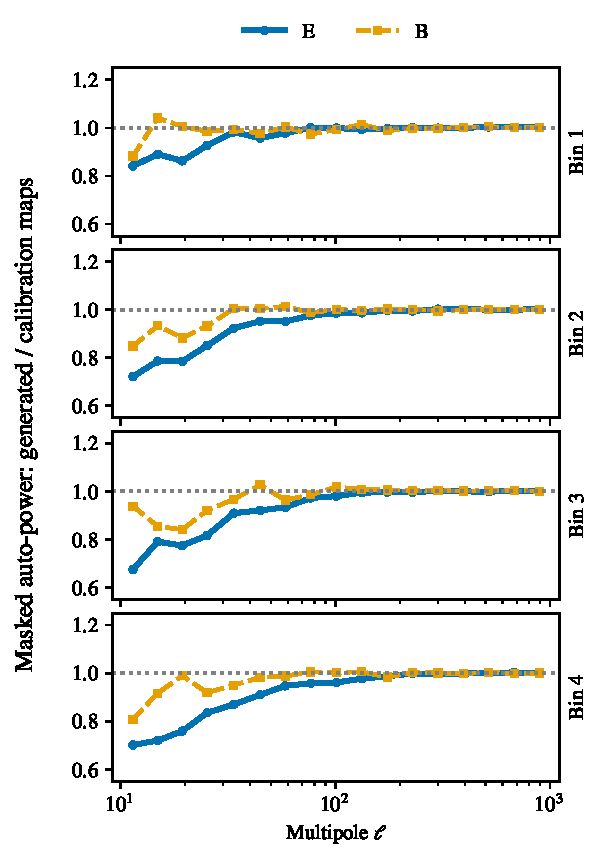
\includegraphics[width=0.66\linewidth]{plots/spectra/spectra.pdf}
 \caption{Generated masked auto-power divided by the 32-map calibration
 measurement. The dotted horizontal line denotes equality.}
 \label{fig:gptg-power}
\end{figure}

\paragraph{Compare the same raw covariance with the full supplied ensemble.}
The direct reference uses all 15,997 available measured vectors; it is not
restricted to the 32 maps used for this initial fit. For the sixteen raw
moments, generated-to-reference variance ratios range from $0.621$ to
$1.440$. The largest absolute correlation difference is $0.332$.
Figures~\ref{fig:gptg-var} and~\ref{fig:gptg-corr} locate these differences.
The generated covariance itself is estimated from only 64 maps. Even for
one exactly Gaussian observable, its sample variance would have fractional
standard deviation
\begin{equation}
 \sqrt{\frac{2}{64-1}}\simeq0.178.
\end{equation}
Non-Gaussian observables need not follow that estimate. We therefore do not
interpret every difference as established model bias, or interpret a noisy
agreement as validation. This pilot shows a practical generator and a
measurable comparison; it does not establish a trustworthy DES covariance.
\begin{figure}[htbp]
 \centering
 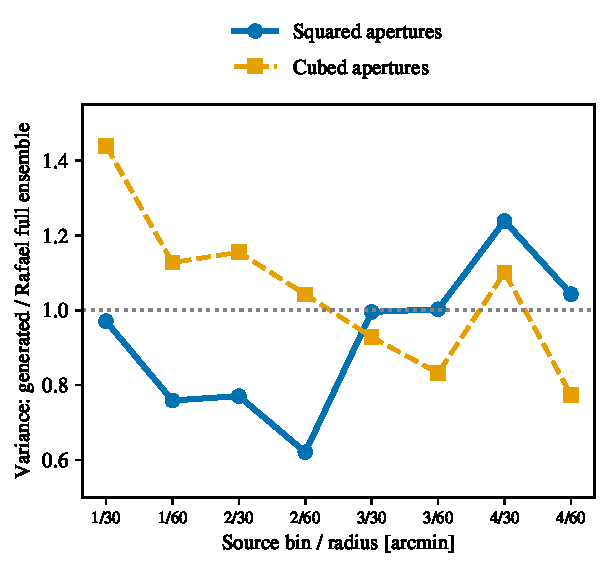
\includegraphics[width=0.72\linewidth]{plots/variance/variance.pdf}
 \caption{Variance ratios for the same sixteen raw moments. The reference
 uses the complete supplied ensemble; the generated estimate uses 64 maps.}
 \label{fig:gptg-var}
\end{figure}
\begin{figure}[htbp]
 \centering
 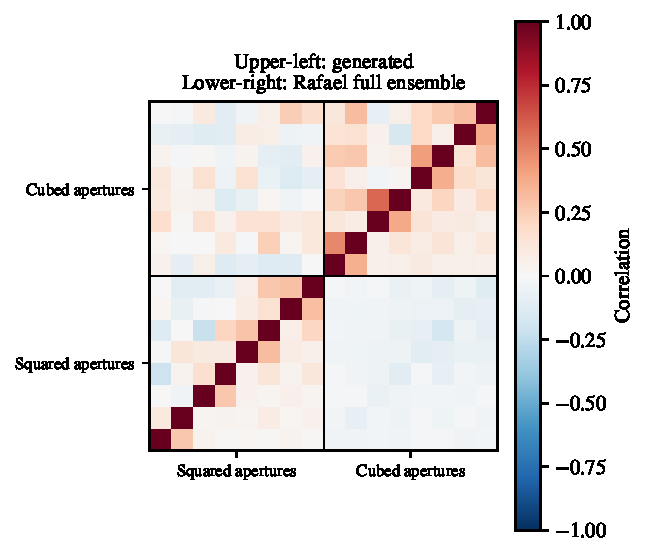
\includegraphics[width=0.7\linewidth]{plots/correlation/correlation.pdf}
 \caption{The two covariance correlations in opposite triangles, with
 their shared second-/third-order row boundary marked.}
 \label{fig:gptg-corr}
\end{figure}

\paragraph{Separate numerical checks from physical matching.}
For the fitted parameters, increasing Gaussian quadrature from 160 to
240 nodes changes the normalized transform by a weighted RMS below
$7.1\times10^{-12}$. The 64-term Hermite relation agrees with direct
bivariate Gaussian quadrature within $5.9\times10^{-12}$ at the checked
correlations; extending to 96 terms changes it by less than
$4.5\times10^{-13}$. A separate band-limited spherical round trip at low
resolution has relative error below $4.9\times10^{-12}$. These checks
support the implemented algebra and transform conventions. They do not
bound errors from the chosen multipole cutoff, masked reconstruction,
noise approximation, calibration sample or absent physical correlations.
The production nonlinear map is not band-limited: projecting it back to a
finite harmonic range discards high-frequency content. A solver residual
in that projection must not be confused with the small band-limited
round-trip error.

\section{Testing sixth-order precision formulas on measured map vectors}
\paragraph{Define a population whose truth can be computed exactly.}
The continuous fitted map model does not come with an exact analytic
covariance for our measurements. To test estimator algebra without guessing
that truth, take the 64 measured vectors as a fixed list. Select four rows:
the squared and cubed 30-arcminute apertures in source bins one and four.
Give every list member probability $1/64$. We now have a discrete probability
model with a known covariance. This is a conditional test on the measured
list, not a claim of 64 perfectly representative N-body skies.

\paragraph{Compute that covariance with the population denominator.}
Let $x_r$ be a four-component list member. Its mean is
\begin{equation}
 \mu=\frac1{64}\sum_{r=1}^{64}x_r.
\end{equation}
The stipulated population covariance is
\begin{equation}
 C_{\rm list}=\frac1{64}\sum_{r=1}^{64}(x_r-\mu)(x_r-\mu)^{\mathsf T}.
\end{equation}
Here the denominator is 64 because the list defines the entire probability
model. When we later draw an independent sample from this model and estimate
its covariance, that sample uses the usual denominator $N-1$.
This distinction prevents a small normalization error from masquerading as
bias in a sixth-order estimator.

\paragraph{Make independent experiments by sampling with replacement.}
For each draw, choose an integer uniformly between zero and 63 and select
that list member. Return it to the list before the next choice. Returning
it allows repeated values while keeping successive choices independent.
For each of 8,192 experiments, draw either 128 or 512 vectors this way.
We use all list members in the probability model, with no calibration or
validation groups. Reusing list members does not create new physical maps;
it creates independent random experiments within a precisely specified
discrete distribution.

\paragraph{Fix the starting matrix before those experiments.}
We first standardize the four measurement coordinates using fixed list
scales. In those coordinates choose
\begin{equation}
 M=2C_{\rm list}+0.1I.
\end{equation}
This deliberately imperfect but positive reference is held fixed for every
resampled experiment. The exact whitened population covariance determines
the second-, fourth- and sixth-order polynomial targets. Its exact inverse
is a separate target. We measure error about both, because removing
finite-sample bias from a polynomial does not make the polynomial equal
to the full inverse.

\paragraph{Read the error comparison rather than choosing the largest order.}
Figure~\ref{fig:gptg-precision} shows relative RMS matrix error about the
exact inverse. For the distribution-independent distinct-pair construction,
the errors at 128 draws are approximately $0.194$, $0.226$ and $0.267$ at
orders two, four and six. At 512 draws they become $0.158$, $0.116$ and
$0.130$. More draws help, and fourth order becomes useful in this example;
sixth order still does not beat fourth. The Gaussian-formula curves are
included as an assumption test. These measured non-Gaussian vectors do not
satisfy a Wishart proof merely because the formula returns a positive matrix.
At 128 draws, the largest mean discrepancy from its sixth-order truncated
target is about $4.8$ Monte Carlo standard errors for that formula. The
corresponding distinct-pair discrepancy is about $2.7$, across the inspected
matrix entries. These are measured diagnostics, not fitted success criteria.
\begin{figure}[htbp]
 \centering
 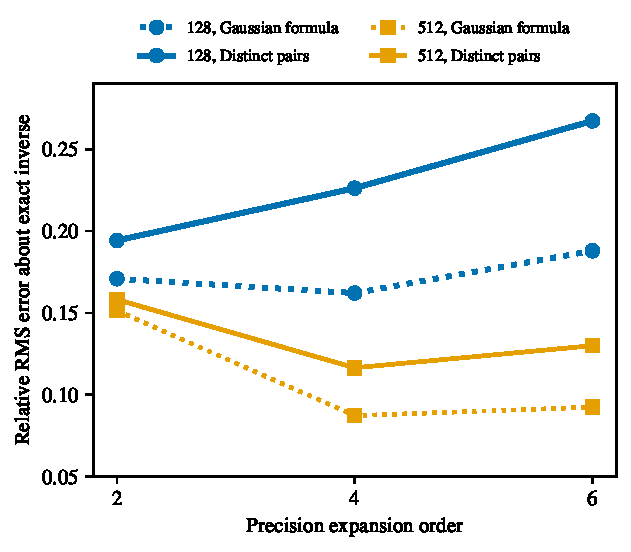
\includegraphics[width=0.75\linewidth]{plots/precision/precision.pdf}
 \caption{Precision errors in independent resamplings of the fixed
 64-member measurement population. New resamplings are not new physical skies.}
 \label{fig:gptg-precision}
\end{figure}
\FloatBarrier

\section{Cost, storage and the next scientific decision}
\paragraph{A measured construction cost.}
Before calibration, three four-bin NSIDE 512 generations with multipoles
through 1024 took approximately 4.28, 3.71 and 4.09 seconds with four
workers. They included scalar synthesis, the point transform, iterative
harmonic analysis, spin-two synthesis and footprint selection. That
benchmark used illustrative spectra and parameters with no shape noise.
It is not a forecast of the complete published three-point measurement
cost. The calibrated 64-map run has median generation-plus-save-plus-aperture
time of 4.27 seconds per map. Extrapolating that measured median gives about
71 minutes for 1,000 maps or 11.9 hours for 10,000; these are extrapolations,
not completed large-ensemble timings. Published triangle measurements can
have a different cost. The run records all three stages separately.

\paragraph{Saving maps is affordable for a pilot.}
The output contains four bins, two components and 369,190 pixels. At eight
bytes per value, the payload size is
\begin{equation}
 4\times2\times369190\times8=23628160\ \mathrm{bytes}.
\end{equation}
Sixty-four maps need about 1.51 GB in decimal units. Ten thousand need
about 236 GB before headers and auxiliary files. The original pilot remains float64 as a precision reference. The measured
rounding check below supports float32 for new saved maps, halving those
storage values while keeping all arithmetic in float64.
The raw maps and generated outputs are ignored by Git; the notes, scripts,
notebook and compact validation evidence belong in the repository.

\paragraph{Decide from measurements rather than file count.}
We must compare spectra, reconstructed distributions, raw and noise-corrected
moments, covariance diagonals, correlations and parameter-sensitive matrix
directions. Matching the one-point distribution and two-point correlation
alone does not establish the four-, five- and six-field correlations needed
by a joint covariance. More generated maps reduce random uncertainty in
those comparisons; they do not remove a persistent disagreement.

\paragraph{How this connects to sixth-order Eifler corrections.}
The separate precision-expansion note derives second-, fourth- and
sixth-order estimators and distinguishes truncation error from sampling
noise. A calibrated generator could provide a more accurate starting
covariance, or a cheap ensemble for testing the estimators. If fitted
using the same finite N-body sample later used for a correction, that
dependence must be accounted for. We cannot invoke a proof conditional
on an independently fixed model while silently fitting that model to the
correction sample. This is a statistical accounting requirement, not a
reason to avoid the generator experiment.

\paragraph{Reproduce the bounded checks without generating another ensemble.}
The companion notebook, \texttt{EXAMPLE\_GPTG\_SIMULATIONS.ipynb}, reads
compact frozen measurements from the repository. Its explicit optional
switches run calibration, map generation or precision resampling. To run
the deterministic numerical checks directly, use
\begin{lstlisting}
check_numerics()
\end{lstlisting}
To repeat the measured-list precision experiment, use
\begin{lstlisting}
map_precision_tests()
\end{lstlisting}
The \texttt{tests/gptg\_pilot/} records retain the actual parameters, row
labels, measurements, timing and numerical checks. The raw generated maps
remain under \texttt{chains/gptg\_method/maps/} and are not committed.

\paragraph{What would justify a larger production ensemble.}
First replace or test the masked-spectrum approximation with a forward
window calculation, and compare both auto- and cross-bin spectra. Fit the
point-function parameters through the same noisy reconstruction used on
the real inputs, rather than identifying a noisy proxy distribution with
the underlying convergence distribution. Obtain the producer's shear basis,
noise and weighting conventions; our sign diagnostic favors the current
component choice but does not replace that information. Then refine the
harmonic cutoff and pixel treatment and measure the actual intended
second-/third-order estimator. Finally propagate uncertainty of the fitted
parameters and examine covariance eigen-directions, not only diagonal
variances. Additional generated mocks become useful for physical forecasts
when those comparisons support the fitted model at the required precision.

\section{A larger ensemble with genuinely separate validation draws}
\paragraph{Freeze the model before testing estimators.}
The authorized larger run has 10,000 comparison maps and 5,000 additional
validation maps. Its generation is in progress at the time of this note;
no results from those 15,000 maps are claimed here. The fitted parameters
are copied once into the run directory, and the two map groups use disjoint
seed ranges, also distinct from the 64-map pilot. Independence here is
conditional on that fixed fitted model. It is not proof that the model
reproduces independent N-body skies.

\paragraph{Use all comparison maps in both estimates.}
The direct covariance and each Eifler estimate use the same 10,000 measured
vectors. The initial reference is fixed in advance to twice the archived
Gaussian raw-aperture reference. The factor of two is a stated benchmark
choice, not fitted using the new comparison or validation maps. Both Gaussian
matrix-power and distinct-pair constructions are tested at orders two,
four and six. Every predeclared result is retained, including a report when
an estimate is indefinite. The 5,000 validation maps do not choose the
reference, order or discarded cases.

\paragraph{The direct inverse is a comparator, not known truth.}
More simulated maps reduce its sampling uncertainty, but inversion can
amplify noise in weak covariance directions. Agreement with a sample inverse
is especially limited evidence when the alternative uses the same sample.
A higher-order polynomial can approach that particular inverse while
reproducing more sample noise. The validation group provides an additional
question: which proposed precision better predicts new fluctuations?

\paragraph{Define a score that never inverts the validation covariance.}
For a fixed positive precision $\Psi$, define
\begin{equation}
 J(\Psi)=\operatorname{tr}(\Psi C_*)-\log\det\Psi,
\end{equation}
where $C_*$ is the unknown covariance of the fitted generator. Lower is
better. This is the covariance-dependent part of an expected Gaussian
quadratic loss. Its optimum is the true inverse covariance even if the
vectors are not Gaussian, provided their covariance exists. It does not
assert that a Gaussian likelihood describes every aspect of those vectors.

\paragraph{Show why its optimum is the true inverse.}
Use the symmetric positive square root of $C_*$ to define
\begin{equation}
 A=C_*^{1/2}\Psi C_*^{1/2}.
\end{equation}
Cyclic invariance of the trace gives
\begin{equation}
 \operatorname{tr}(\Psi C_*)=\operatorname{tr}(A).
\end{equation}
Multiplication of determinants gives
\begin{equation}
 \det A=\det C_*\,\det\Psi.
\end{equation}
Taking logarithms and solving for the precision determinant gives
\begin{equation}
 \log\det\Psi=\log\det A-\log\det C_*.
\end{equation}
Substitute these two identities into the score:
\begin{equation}
 J(\Psi)=\operatorname{tr}(A)-\log\det A+\log\det C_*.
\end{equation}
The last term does not depend on the candidate precision. If $\lambda_i$
are the positive eigenvalues of $A$, the remaining terms are
\begin{equation}
 \sum_i\left(\lambda_i-\log\lambda_i\right).
\end{equation}
For one positive number, the derivative of $x-\log x$ is $1-1/x$.
It vanishes at $x=1$; its second derivative is $1/x^2>0$. Each eigenvalue
therefore minimizes the score at one. Thus $A=I$ is the optimum. Multiplying
that identity on each side by $C_*^{-1/2}$ gives
\begin{equation}
 \Psi=C_*^{-1}.
\end{equation}
We have established the target of the score without using an observed
sample inverse as the truth.

\paragraph{Estimate the score difference on independent maps.}
Let $r_a$ be a validation vector minus the validation sample mean. Its
ordinary sample covariance is
\begin{equation}
 \widehat C_v=\frac1{N_v-1}\sum_{a=1}^{N_v}r_ar_a^{\mathsf T}.
\end{equation}
For the candidate precision and the direct comparison-sample precision,
define their fixed difference
\begin{equation}
 D=\Psi-\Psi_{\rm direct}.
\end{equation}
The measured score difference is
\begin{equation}
 \widehat{\Delta J}=\operatorname{tr}(D\widehat C_v)
             -\log\det\Psi+\log\det\Psi_{\rm direct}.
\end{equation}
Insert the sample-covariance sum into its trace term:
\begin{equation}
 \operatorname{tr}(D\widehat C_v)
 =\frac1{N_v-1}\sum_a\operatorname{tr}(Dr_ar_a^{\mathsf T}).
\end{equation}
For a column vector, cyclically moving the factors inside the trace leaves
a one-by-one matrix. Its trace is just its scalar value:
\begin{equation}
 \operatorname{tr}(Dr_ar_a^{\mathsf T})=r_a^{\mathsf T}Dr_a.
\end{equation}
We can therefore calculate the comparison directly from new realizations,
without inverting their covariance. A negative measured difference favors
the candidate on this validation sample. Its uncertainty comes from the
scatter of the quadratic differences; the reported standard error is an
asymptotic estimate, since centering by a sample mean introduces weak
within-group dependence. Indefinite precisions receive no such score.

\paragraph{Storage precision is tested separately from arithmetic precision.}
The storage-only test used float64 generation and transforms, with
float32 saved maps. The later production run also uses tested float32
arithmetic on some workers, as described in Section~\ref{sec:sht-teaching}.
Covariance and inversion remain float64. Saved pixels are decoded to float64 before measuring the recorded
vectors. This ensures the journal can be reproduced from the files later
read by a student. The 64 original pilot maps remain float64 solely as a
small precision-test reference.

\paragraph{Measure the rounding error on actual observables.}
For each pilot map we rounded its pixels to float32, decoded them to
float64, and repeated the same filtering and moment calculation. Across
all 64 maps, the largest absolute shear change was $8.58\times10^{-9}$.
The largest joint covariance-weighted vector change was
$2.56\times10^{-7}$. The largest fractional variance change was
$1.50\times10^{-8}$; the largest relative covariance or precision change
in any matrix direction was about $5.25\times10^{-8}$. These effects are
negligible for the tested 30/60-arcminute diagnostics. A cubic moment near
zero is not a useful denominator for a relative-error check, so we compare
against the measured covariance and its matrix directions instead.

\paragraph{Retain maps without doubling the working disk.}
Fifteen thousand float32 maps require about 177 GB. The runner writes one
map at a time, keeps a 50 GB free-space reserve, and flushes a text journal
after every completed map. A temporary file is renamed only after a map
save completes; full-sky intermediates stay in memory. Restarting the same
command resumes completed records instead of regenerating them:
\begin{lstlisting}
mpirun -n 1 python projects/des_3pcf/scripts/generate_ensemble_mpi.py --threads 4
\end{lstlisting}
The serial command above is available for small runs. The current large
run instead uses MPI with three CPU workers and one GPU scalar-transform
worker, each with three CPU transform threads, plus a coordinator. BLAS
remains one. Local generation is now paused at the user's request. Previously
saved maps are preserved, and the numerical-mode history records changes
in worker allocation and arithmetic. Section~\ref{sec:sht-teaching}
explains the transforms and the numerical checks for the GPU path.
Completion verification checks all expected IDs, seeds, file shapes and
sizes; it does not claim a full scan of every saved pixel. Analysis is a
separate step. A validation preference is a result to report, not permission
to tune repeatedly against the same validation group.

\section{Measuring the full joint vector from saved maps}
The main covariance experiment uses TreeCorr 5.1.2, credited to Mike Jarvis
and contributors. \texttt{GGCorrelation} produces 400 $\xi_\pm$ entries:
ten source-bin pairs, twenty angular bins and two shear correlations.
\texttt{GGGCorrelation}, followed by \texttt{toSAS()} and
\texttt{calculateMap3()}, produces 80 equal-filter third-order entries:
twenty source-bin triples and four aperture radii. These measurements
replace the small aperture diagnostic as the science comparison.

The updated TreeCorr build supports OpenMP. For multi-node measurement,
mpi4py and Open MPI assign each ready map to one worker, which completes
its unfinished tomographic tasks;
CPU allocations must count both MPI ranks and native threads. A separate
coordinator receives results and writes small text vectors. The downloaded HPC measurements are investigated below; neither map
generation nor a new TreeCorr run is started by this investigation.
BLAS is one per process. The measurement keeps every two-/three-point
cross entry, while the analytical 400-by-400 G+SSC+cNG block stays fixed.

Section 13 of the covariance teaching note gives the precise triangle cuts,
row ordering, starting covariance and correction algebra. It distinguishes
NSIDE512 equal-pixel measurements from the published catalogue estimator.
The initial first-1,000-map plan is superseded by the all-complete-vector
comparison in Section~\ref{sec:joint-audit}. The older sixteen-entry tests
are algebra demonstrations, not answers for the full measurement.

\section{Investigation of the downloaded joint measurements}
\label{sec:joint-audit}
\paragraph{Qualification added after the measurement review.}
The figures in this section use the legacy mixed-source measurement.
Section~\ref{sec:review-repair} identifies its self-product error and
explains the repair. These results diagnose the saved vectors; they are
not a validated covariance comparison for the intended observable.
\paragraph{The target of this experiment.}
Our immediate question is whether a precision expansion estimates the
covariance of the Kunhao-generated ensemble better than a direct sample
calculation. Reproducing Rafael's published covariance is a different
question. New random seeds generate independent maps conditional on the
chosen calibration. Fitting that calibration to Rafael's maps does not
invalidate this conditional experiment. The comparison below uses all
complete downloaded vectors for both methods; it does not divide them
into calibration, correction and validation groups.

\paragraph{Begin with the saved measurements.}
The 22 November investigation found 1,878 complete vectors: map IDs
0--938 and 5000--5938. It excluded 1,878 partial checkpoints and counted
any repeated complete ID only once, after checking equality. Each stored
vector has 480 positions. A position in a file, however, is not necessarily
a measured random variable. We must check that its angular bin actually
contains pairs before interpreting its variance.

\paragraph{Why sixty entries are identically zero.}
The catalogue given to TreeCorr contains one position per retained
NSIDE512 pixel. A nearest-neighbor calculation on the actual footprint
finds the minimum distinct-pixel separation
\begin{equation}
 \theta_{\mathrm{nearest}}=5.6134446\ \mathrm{arcmin}.
\end{equation}
The first three requested angular intervals are
\begin{equation}
 [2.5,3.1473],\quad[3.1473,3.9622],\quad[3.9622,4.9882]
 \quad\mathrm{arcmin}.
\end{equation}
Every upper edge is smaller than the minimum separation. Consequently
these intervals contain no distinct pairs. Direct counting of positions,
without running TreeCorr, gives zero pairs in all three intervals. The
next interval contains 75,869 unordered pairs, followed by 578,948 in the
following interval. The abrupt change illustrates how discrete pixel
geometry differs from a continuously sampled annulus.

\paragraph{A missing measurement is not a measured zero correlation.}
There are ten source-bin pairs and two shear correlations. Repeating
three empty intervals for each produces
\begin{equation}
 3\times10\times2=60
\end{equation}
constant zero entries. Their sample covariance has zero rows and columns,
so the full 480-dimensional sample covariance has no inverse. The runner
checked that entries were finite, but did not distinguish an empty-bin
zero from a measured value. This is a measurement-configuration failure
that should have been detected before the large run. It does not show
that the saved shear maps are corrupt. Interpolating them to more pixel
centers would not create the unresolved signal or independent galaxy noise.

\paragraph{What can still be studied.}
We retain the complete vectors and explicitly select their 420 varying
entries: 340 two-point entries and 80 third-order entries. The notebook
checks that the removed rows are exactly those predicted by geometry;
it does not discard other inconvenient modes. The selected sample
covariance is positive definite. That establishes the existence of its
inverse, not convergence to the population covariance. The remaining
small-angle measurements still have discrete angular weights; removing
empty bins alone does not establish agreement with a catalogue estimator.

\paragraph{Both fixed-block methods must use the same block.}
Write the ordinary sample covariance of the selected vector as
\begin{equation}
 S=\begin{pmatrix}S_{xx}&S_{xy}\\S_{yx}&S_{yy}\end{pmatrix}.
\end{equation}
For the experiment in which the analytical two-point block $A$ is
stipulated exact, the direct comparison with a fixed-$A$ expansion is
\begin{equation}
 C_h=\begin{pmatrix}A&S_{xy}\\S_{yx}&S_{yy}\end{pmatrix}.
\end{equation}
We keep $A$ unchanged. Comparing only an unconstrained $S$ with a
constrained estimate would mix a change in the two-point block with the
change in covariance estimator. The notebook therefore shows both $S$
and $C_h$, and explains which comparison each serves. If the supplied
$A$ differs from this generator's two-point covariance, $C_h$ is a
stipulated hybrid target, not the full covariance of the original random
vector. This distinction does not question the accuracy of the analytical
calculation for its own specified survey.

\paragraph{Check that the fixed-block target is possible.}
With $A$ positive definite, the remaining condition is positivity of
its Schur complement. Compute it by solving a linear system:
\begin{equation}
 AU=S_{xy}.
\end{equation}
Then subtract the part of the third-order covariance accounted for by
its correlation with the two-point vector:
\begin{equation}
 C_{y\mid x}=S_{yy}-S_{yx}U.
\end{equation}
Its smallest eigenvalue in starting-Map3-covariance units is 0.360 in
this sample. It is positive. Thus the failed precision corrections below
are not explained by an intrinsically impossible fixed-$A$ sample target.
No negative eigenvalues were clipped to obtain this result.

\paragraph{Identify the actual starting covariance.}
The starting matrix is
\begin{equation}
 M=\begin{pmatrix}A&0\\0&D_0\end{pmatrix}.
\end{equation}
Here $A$ is the production Gaussian+SSC+cNG covariance, whereas $D_0$
comes from the released simulation covariance FITS file. This matrix
must not be described as a fully analytical joint covariance. The FITS
row labels match our source-bin ordering, and all three aperture radii
match the equal-filter radii used by the runner. These checks exclude a
simple row-order error, but do not establish that $D_0$ approximates the
Kunhao-generated ensemble.

\paragraph{The generated maps include shape noise.}
Both the CPU and GPU production paths add independent Gaussian noise
per shear component, source bin and pixel. Earlier discussion that called
these production maps noiseless was incorrect; noiseless maps occur only
in separate numerical comparison tests. The amplitudes are recorded in
\texttt{calibration.npz}. For comparison, a uniform galaxy-density model
would imply a pixel noise variance
\begin{equation}
 \sigma_{\mathrm{pixel},i}^{2}
 =\frac{\sigma_{e,i}^{2}}{n_i\Omega_{\mathrm{pixel}}}.
\end{equation}
The denominator is the expected number of galaxies in a pixel. The actual
fitted noise variances divided by this expression from the analytical
settings are 1.476, 1.502, 1.519 and 1.579. The equal-pixel footprint covers
4841.54 square degrees; the analytical settings use 4143 square degrees.
These are different experimental specifications. A precise covariance
for one specification is not automatically the covariance of the other.

\paragraph{A large mismatch in the third-order reference.}
Across the 80 third-order variances, the sample variance divided by
$D_0$'s corresponding diagonal ranges from 3.84 to 37.49. Its median is
about 11.6. The dependence on aperture radius is explicit:
\begin{center}
\begin{tabular}{rrrr}
\toprule
Radius [arcmin]&Minimum ratio&Median ratio&Maximum ratio\\
\midrule
7 &13.53&16.96&37.49\\
14&13.57&17.49&24.68\\
25&4.30&6.74&10.14\\
40&3.84&5.68&8.93\\
\bottomrule
\end{tabular}
\end{center}
These are comparisons of measured variances, not correction factors to
apply to data vectors. Noise and area differences do not by themselves
explain the whole table. The initial generator fit, angular resolution,
triangle weights and finite multipole reconstruction remain possible
contributors. Assigning the excess to one of them without a matched
measurement test would go beyond the evidence.

\paragraph{The expansion fails before considering noisy products.}
Take the Cholesky factor of the reference:
\begin{equation}
 M=LL^{\mathsf T}.
\end{equation}
Measure the stipulated target in reference units:
\begin{equation}
 W=L^{-1}C_hL^{-\mathsf T}.
\end{equation}
Define its departure from the identity by
\begin{equation}
 E=I-W.
\end{equation}
The desired inverse in these units is
\begin{equation}
 W^{-1}=(I-E)^{-1}.
\end{equation}
For an eigenvector of $E$ with eigenvalue $e$, this reduces to the scalar
problem of approximating $1/(1-e)$. Multiplying a finite geometric sum
makes every interior term cancel:
\begin{equation}
 (1-e)(1+e+e^2+\cdots+e^q)=1-e^{q+1}.
\end{equation}
Divide by $1-e$ and subtract the desired inverse:
\begin{equation}
 \sum_{j=0}^{q}e^j-\frac{1}{1-e}
 =-\frac{e^{q+1}}{1-e}.
\end{equation}
Finally divide by $1/(1-e)$ to obtain the relative inverse error:
\begin{equation}
 \epsilon_q=-e^{q+1}.
\end{equation}
It tends to zero only when $|e|<1$. Our sample diagnostic gives eigenvalues
from $-58.5985$ to $0.8760$. The largest magnitude is far outside that
range. More maps reduce sampling error around the generator's covariance;
they do not make a badly chosen starting matrix approach it.

\paragraph{Why simply inflating the reference is insufficient.}
As a diagnostic, we multiply only $D_0$ by fixed trial factors and repeat
the deterministic sample calculation. These choices were inspected after
seeing the data; they are not independently specified PME estimates. Even
a factor of 32 leaves an eigenvalue of $W$ near 2.39, outside the interval
$(0,2)$ needed for convergence. A factor of 64 puts the sample spectrum
inside that interval, but its smallest eigenvalue is about 0.00552.
The corresponding sixth-order relative error has magnitude about 0.962.
The series now converges eventually, yet six terms beyond the identity
are nowhere near sufficient in that direction. A useful low-order
reference must describe covariance directions as well as overall scale.

\paragraph{Test the implementation separately from the reference.}
The notebook's distinct-independent-pair recurrence agrees with explicit
enumeration of matrix products through degree six. A small repeated
Gaussian experiment checks its mean against the deterministic polynomial.
For a further control with 1,878 draws and 420 dimensions, the reference
is set to the exact identity covariance and its leading 340-dimensional
block is fixed. The minimum conditional-precision eigenvalues at orders
2, 4 and 6 are respectively 0.378, 0.371 and 0.143: all positive in this
seeded control. This checks a relevant numerical regime. One such control
does not establish estimator accuracy or positivity for every realization.

\paragraph{What fails on the measured vectors.}
The corresponding minimum conditional-precision eigenvalues for the
actual vectors, in the original reference units, are approximately
$-2.53$, $-1.69\times10^5$ and $-2.09\times10^9$. None defines a covariance
through the conditional construction. Unbiased estimation of a finite
matrix polynomial does not guarantee positivity in each realization.
Our estimator uses distinct pair factors in their original order, so
individual estimates also depend on pairing and order. It is an extension
of the precision-expansion idea, not the original paper's Gaussian
second-order formula. Its final fixed-$A$ reconstruction is nonlinear
and is not claimed unbiased. These qualifications must accompany any
future performance comparison.

\begin{figure}[htbp]
\centering
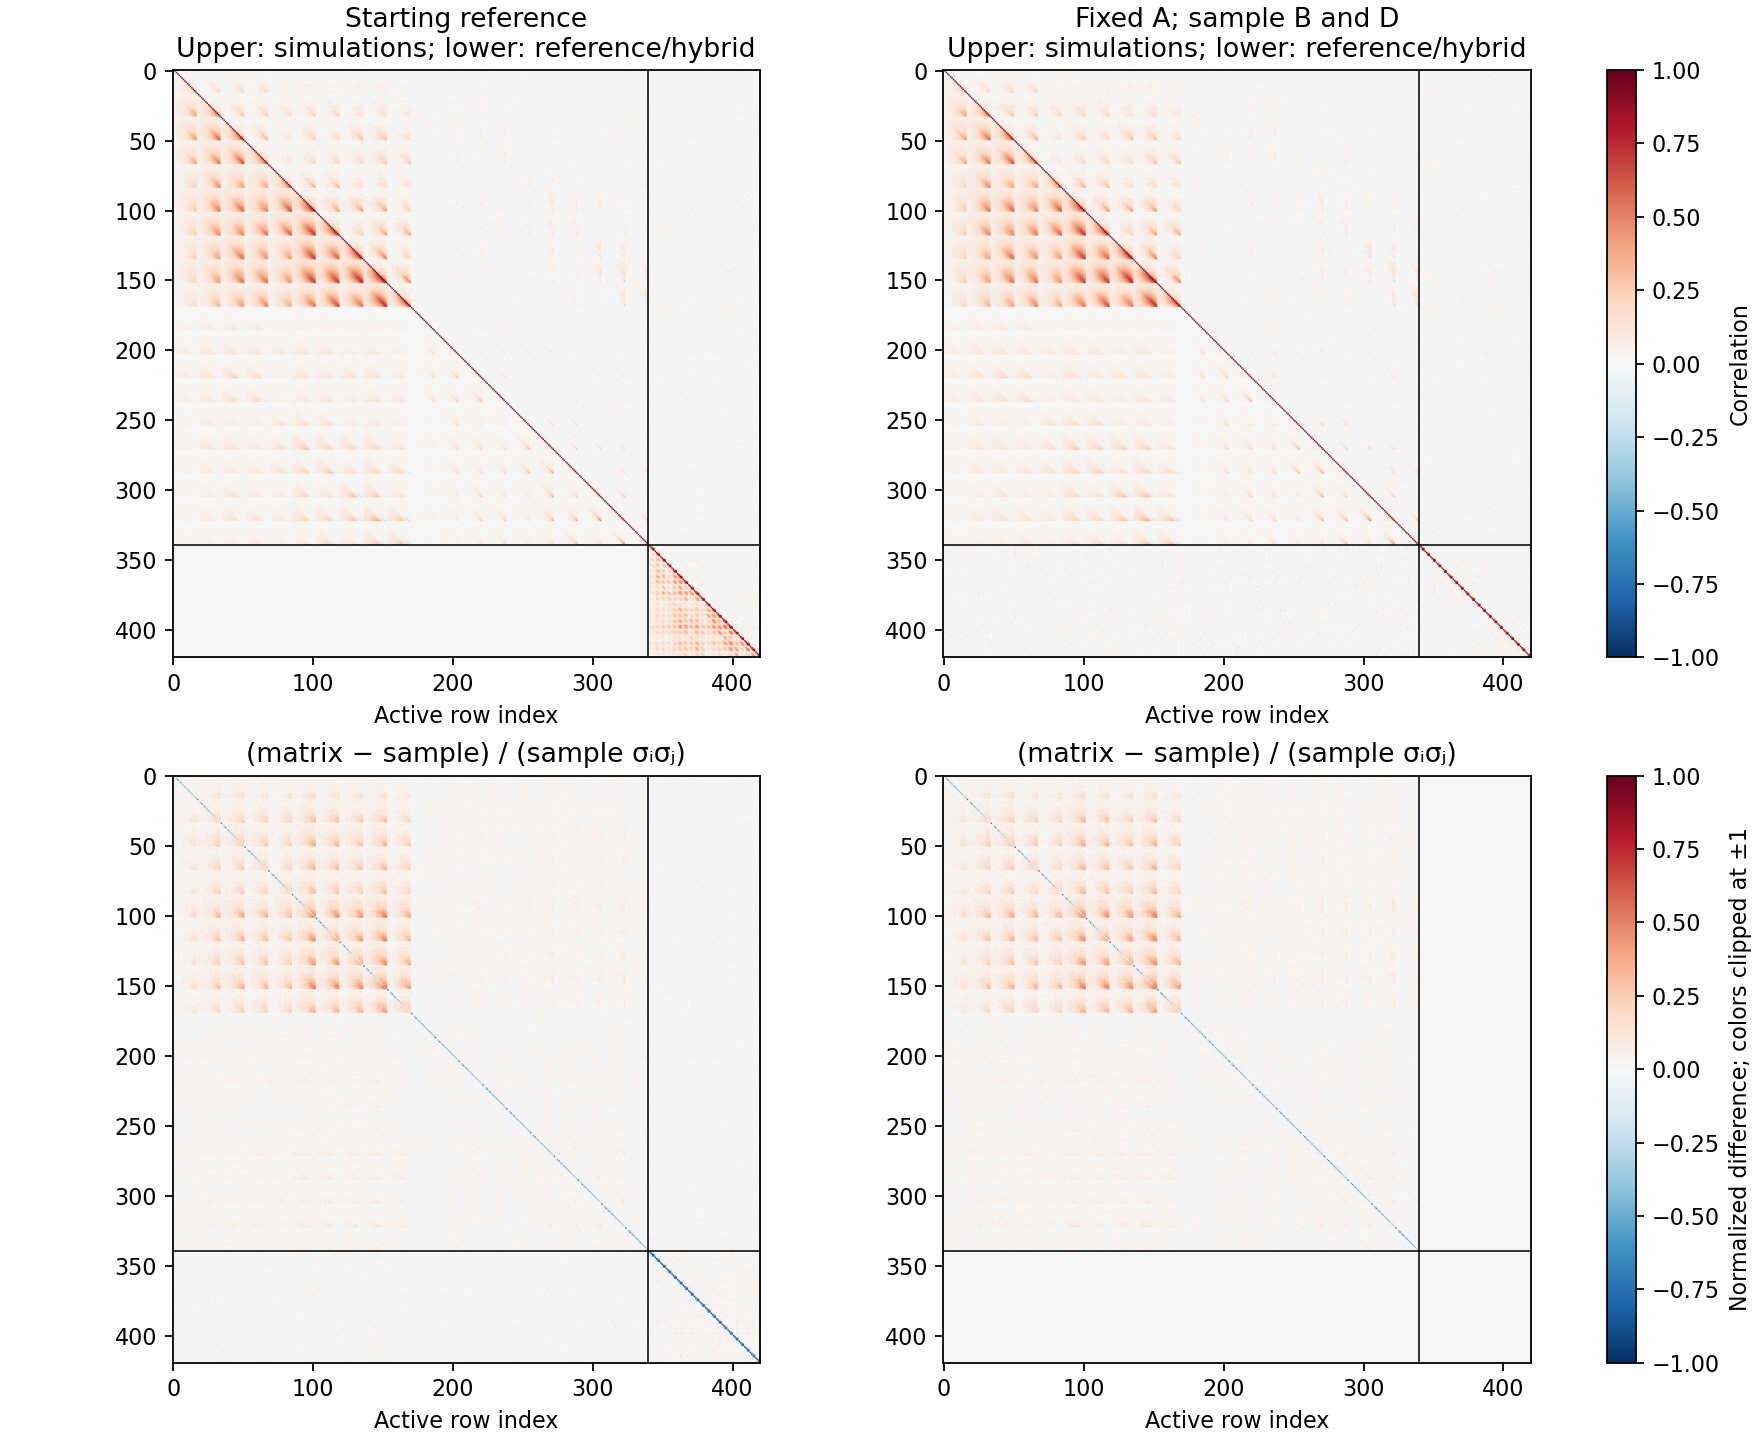
\includegraphics[width=\linewidth]{plots/full_joint_audit/comparison.png}
\caption{The varying rows only. Upper triangles show the direct sample;
lower triangles show either the starting reference or fixed $A$ with
sample cross and third-order blocks. Differences use the same sample
standard deviations in both panels. These are not PME covariance plots:
no valid PME covariance was obtained in this run.}
\end{figure}
\begin{figure}[htbp]
\centering
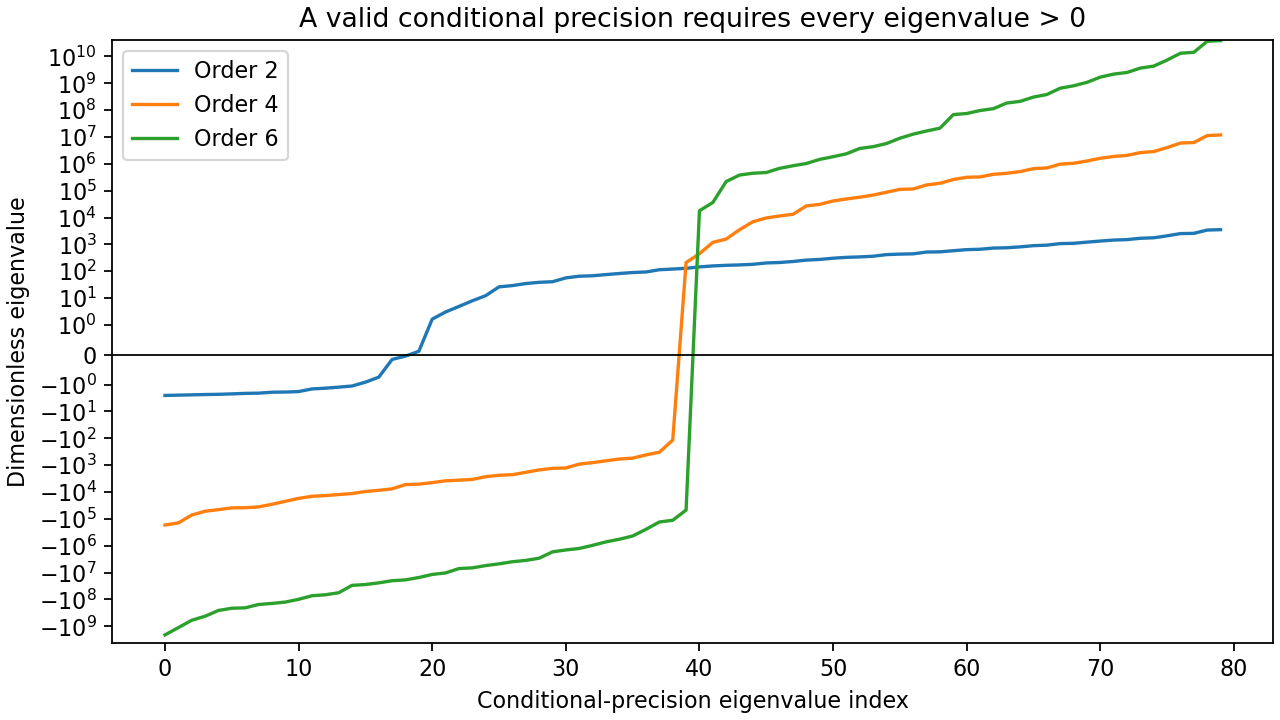
\includegraphics[width=0.94\linewidth]{plots/full_joint_audit/precision_eigenvalues.png}
\caption{Signed conditional-precision eigenvalues. A negative eigenvalue
invalidates the proposed covariance. The vertical scale is logarithmic
away from zero and linear near zero, so both signs remain visible.}
\end{figure}
\FloatBarrier

\paragraph{What the published measurement comparison establishes.}
Gomes et al.~\cite{gomes} use NSIDE1024, with galaxy-position noise before
pixel averaging. Their roughly eight-arcminute lower triangle-side cut
was checked at that resolution. It cannot be assumed validated at our
coarser NSIDE512 resolution. The file supplied here also records
\texttt{NSIM=500}, whereas the paper describes 796 footprints; the lineage
of this particular covariance should be confirmed before using its
simulation count in a likelihood. Neither issue makes Rafael's result
inconsistent: our measurement and this specific archived file need to
be identified correctly. For the present estimator benchmark, no exact
reproduction of that published experiment is required.

\paragraph{The next decision is about the benchmark, not more map count.}
Retain the maps and completed measurements. Use the same selected rows
and the same fixed $A$ on both sides of the estimator comparison. Develop
a positive reference close enough to this generated ensemble's stipulated
covariance that low-order truncation is actually small. References chosen
using the correction data need their dependence acknowledged; they cannot
inherit an independent-reference unbiasedness claim automatically. Before
resuming a large measurement allocation, decide whether the supported
pixel-scale observable is the intended benchmark. For subsequent DES
interpretation, small matched Rafael/GPTG measurements should retain pair
and triangle weights and vary angular cuts and multipole truncation.
The existing final-vector checkpoints do not contain those weights, so
they cannot resolve all those questions retrospectively.

\paragraph{A later correction with Rafael's simulations is possible.}
A positive covariance constructed from GPTG can serve as a new reference
for precision expansion using Rafael's maps. The reference need not be
purely analytical. It must describe the same observable and be sufficiently
close for the chosen truncation. The present indefinite PME results cannot
be used for this purpose. Moreover, the calibration uses Rafael parent
runs 0--31. New synthetic random seeds do not remove dependence on those
parents. To apply the independent-reference argument in that second
experiment, use correction parents absent from the fit, or account for
reused calibration information explicitly. Noise rotations and separate
footprints of the same parent are not new independent parents. This is
separate from the immediate conditional Kunhao-ensemble experiment, for
which the new maps are independent draws from the fitted model.

\section{Two further reviews: what the old measurements can establish}
\label{sec:review-repair}
\paragraph{Read this qualification before using the preceding comparison.}
The preceding audit correctly identifies empty angular bins and a failed
precision expansion for its supplied reference. A further review found
an independent error in the mixed-source three-point measurement. Those
legacy vectors therefore cannot establish the performance of covariance
estimation for the intended observable. Keep the original maps: the error
is in measuring them, not evidence of an error in generating them. Existing
two-point results remain available for analysis. New mixed-source results
must use a new measurement directory and definition.

\paragraph{Different source bins can occupy the same pixel.}
Our four source fields share one list of sky positions. The shear in source
bin $a$ and the shear in source bin $b$ can differ at a given position,
but the position itself is identical. In the old three-catalogue multipole
call, products involving this same neighbour were retained. An auto
correlation removes these self products. Merely dropping the zero opening
angle after a truncated Fourier reconstruction is insufficient: a finite
Fourier series spreads a contribution at zero angle into neighbouring
angle bins. Thus a nonzero lower angle cut does not repair this mistake.

\paragraph{Which old entries need reconsideration?}
There are twenty unordered source triples and four aperture radii per
triple. Four triples use a single source bin three times. Their sixteen
entries already used the auto route. The other sixty-four entries used
mixed catalogues with common pixel positions. Tiny spherical tests isolate
the problem for repeated-source triples; the distinct-source triples also
share coincident positions and are included in the repaired definition.
The remaining auto entries still require angular-truncation convergence;
being unaffected by this particular error is not a complete validation.

\paragraph{Recover mixed moments from ordinary auto measurements.}
Let $a$ and $b$ denote complete shear fields, not individual numbers. Write
$P(a)$ for the auto third aperture moment of field $a$. With common
positions and weights, the same triangle counts normalize every combined
field. Equal aperture radii make the associated trilinear operation $T$
symmetric. Expanding the product gives
\begin{equation}
 P(a+b)=P(a)+3T(a,a,b)+3T(a,b,b)+P(b).
\end{equation}
The coefficient three counts the choices of which of the three factors
supplies the different field. Changing $b$ to $-b$ changes terms with an
odd number of $b$ factors:
\begin{equation}
 P(a-b)=P(a)-3T(a,a,b)+3T(a,b,b)-P(b).
\end{equation}
Now subtract the second equation from the first. The pure $a$ terms cancel;
the terms with two $b$ factors cancel as well. The remaining terms are
\begin{equation}
 P(a+b)-P(a-b)=6T(a,a,b)+2P(b).
\end{equation}
Move the last term to the left and divide by six:
\begin{equation}
 T(a,a,b)=\frac{P(a+b)-P(a-b)-2P(b)}{6}.
\end{equation}
For the other repeated-source moment, add the first two equations instead.
This cancels terms with an odd number of $b$ factors:
\begin{equation}
 P(a+b)+P(a-b)=2P(a)+6T(a,b,b).
\end{equation}
Solving for the unknown mixed moment yields
\begin{equation}
 T(a,b,b)=\frac{P(a+b)+P(a-b)-2P(a)}{6}.
\end{equation}
These identities use only auto measurements, so their triangle exclusion
is consistent. They apply to this common-mask, common-weight, equal-radius
runner; they are not a replacement formula for arbitrary galaxy catalogues.

\paragraph{Three different source fields.}
Expand $P(a+b+c)$. It contains three pure cubes, six types of terms with
two source labels, and six permutations with three different labels.
Subtracting $P(a+b)$, $P(a+c)$ and $P(b+c)$ removes all two-label terms.
Each pure cube occurs in two of these subtractions, so its net coefficient
is $1-2=-1$. Adding the three pure cubes back leaves just
\begin{equation}
\begin{split}
 6T(a,b,c)={}&P(a+b+c)-P(a+b)-P(a+c)-P(b+c)\\
            &+P(a)+P(b)+P(c).
\end{split}
\end{equation}
For four source bins we need four single-field autos, six pair sums,
six pair differences and four triple sums: twenty auto calculations in
all. Only their four aperture values are cached for a map. The cache is
cleared when the worker receives another map. The original input shear
sign convention is applied once, before fields are combined.

\paragraph{What the repair tests actually show.}
A small spherical catalogue permits direct triangle enumeration. For
exactly representable test shears, all twenty recovered triples agree
with this independent calculation to a relative norm of
$9.74\times10^{-16}$. Two fresh linear combinations checked against the
actual multipole auto route give relative differences of
$2.02\times10^{-15}$ and $1.12\times10^{-14}$.
These tests check algebra, normalization and signs. They do not establish
that the production angular Fourier cutoff is adequate. TreeCorr also
stores weighted shear internally at single precision; arbitrary floating
inputs need a rounding allowance when comparing a sum of catalogues with
a catalogue of summed shears. An ordinary floating-point fixture gives
$5.99\times10^{-8}$, while shuffled tasks, partial-resume subsets and
cache clearing for a new doubled-shear field pass their exact checks.

\paragraph{Why resuming old mixed results is forbidden.}
A checkpoint contains final aperture values, not all intermediate
correlations. We cannot subtract the unwanted terms retrospectively from
those four values. The repaired runner writes a measurement revision in
both metadata and vector headers. It refuses legacy vectors before writing
new metadata or merging shards. The smoke-pixel setting must also match.
Changing the MPI allocation or requested map count is allowed; changing
the observable while retaining completed entries is not. The old files
remain evidence and are not silently migrated. Map IDs must continue to
refer to immutable input files. Replacing the ensemble requires a fresh
measurement directory even if the estimator revision is unchanged.

\paragraph{An analytical Gaussian three-point reference was also tested.}
The first audit's three-point reference came from a released simulation
covariance. We separately formed a Gaussian full-aperture approximation
from the frozen generator spectra, its pixel-noise level and the measured
footprint area. Gaussian six-point moments contain fifteen pairings:
six pairings link all three fields between aperture centres; nine have
one link and an internal pair at each centre. A circular window of equal
area approximates the footprint. Doubling the integration sampling changes
the covariance by $1.79\times10^{-5}$ in the largest entry normalized by
the corresponding diagonal standard deviations.

\paragraph{Integration accuracy is not estimator agreement.}
This calculation integrates full aperture filters, whereas TreeCorr uses
finite triangle cuts. It lacks the generator's connected higher moments
and does not reproduce the actual irregular window. Its whitened residual
still has an eigenvalue near $-14.92$, outside the convergence interval.
Second-, fourth- and sixth-order corrections to the legacy measurements
remain invalid. The result rules out this particular approximate reference
for these vectors; it does not isolate missing connected covariance as
the cause. The measurement error and the filter difference must be resolved
before making that physical attribution.

\paragraph{A control with a covariance that really is known.}
To separate numerical algebra from uncertain physical truth, consider the
finite population consisting of the saved complete vectors. Define its
mean and covariance using every population member, with denominator $N$.
We then draw from this fixed discrete distribution with replacement.
Conditional on that population, its covariance is known exactly and new
indices are independent draws. Repeatedly selecting an existing vector
creates a new statistical draw from this discrete model; it does not
create a new independent cosmological sky.

\paragraph{Remove the affected mixed-source entries in this control.}
One version retains the 340 supported two-point entries and the sixteen
auto three-point entries, giving 356 dimensions. We change units separately
within each block so their population covariances become identities. This
is a constructed control with an exact two-point block. It neither fits
nor replaces the stipulated production analytical block. A model with a
zero cross block and a three-point block $1.1$ times its exact value has
residual spectral radius $0.537$, so the noiseless series converges.

\paragraph{Separate truncation from sampling.}
For this control the noiseless second-, fourth- and sixth-order polynomials
have root-mean-square relative precision errors of $0.02329$, $0.005135$
and $0.001224$. Higher order therefore removes truncation error as expected.
When the powers are estimated from noisy draws, their variance also enters.
The error we report is
\begin{equation}
 e_{\rm RMS}=\frac{\|L_*^T\widehat\Psi L_*-I\|_F}{\sqrt d},
 \qquad C_*=L_*L_*^T.
\end{equation}
Here $C_*$ is the exact covariance of the chosen discrete population.
The Frobenius norm squares every matrix entry, adds them, and takes a
square root. A correct precision makes the matrix inside the norm zero.
This average error is not a bound on every parameter error or eigenmode.

\paragraph{The direct comparator needs care when $A$ is fixed.}
Replacing the upper-left block of a sample covariance by $A$ gives one
simple hybrid. Even if the original sample covariance is positive definite,
the replacement can violate the Schur condition
\begin{equation}
 S_{yy}-S_{yx}A^{-1}S_{xy}>0.
\end{equation}
Thus a failed hybrid must not be described as a failed ordinary sample
covariance. Another direct estimator uses the sample regression and its
residual covariance:
\begin{equation}
 H=S_{yx}S_{xx}^{-1}.
\end{equation}
This matrix predicts the three-point vector from the two-point vector.
Subtract the covariance explained by that prediction:
\begin{equation}
 V=S_{yy}-S_{yx}S_{xx}^{-1}S_{xy}.
\end{equation}
Rebuild a joint model using the stipulated $A$ for the predictor:
\begin{equation}
 C_{\rm reg}=\begin{pmatrix} A&A H^T\\H A&V+H A H^T\end{pmatrix}.
\end{equation}
Its conditional covariance is $V$. It is positive definite when $A$ and
$V$ are positive definite. It also has sampling bias and variance; positivity
alone does not make it the best estimator. The notebook compares both direct
constructions rather than treating the simple block replacement as the
only possible simulation-based method.

\paragraph{Higher order is not a promise of lower total error.}
In four repetitions of the 356-dimensional control at 4,000 draws, median
RMS errors are $0.1174$ for direct block replacement and $0.1188$, $0.1410$,
$0.1467$ for orders two, four and six. At 40,000 resampled draws they are
$0.03123$, $0.04248$, $0.04260$, $0.04374$. The regression construction
reduces the direct-method errors to $0.10963$ and $0.02847$ at these two
counts, on exactly the same random draws. At 1,878 draws second order
has error $0.17986$, compared with $0.20536$ for regression; the ranking
changes with sample count. These are conditional tests of
one population, reference and estimator implementation. They neither
predict the error from 40,000 new skies nor establish one-percent accuracy.
A quadratic-error ranking can differ from a likelihood-loss ranking.

\begin{figure}[htbp]
\centering
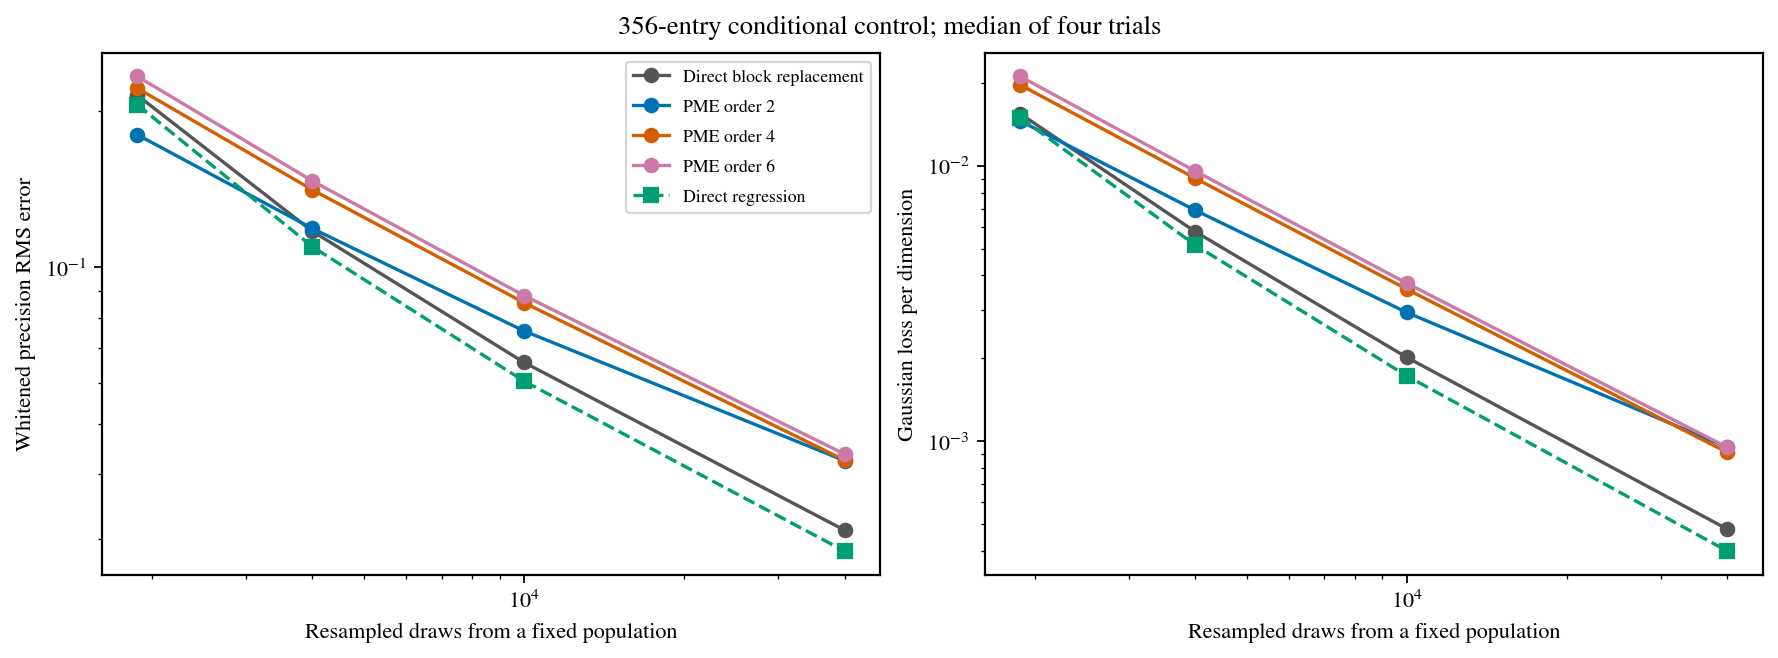
\includegraphics[width=\linewidth]{plots/full_joint_audit/empirical_controls.png}
\caption{Known finite-population control restricted to auto-source Map3
entries. Every method uses the same draws. Four-trial medians describe
this experiment, not an accuracy forecast for new skies. Left: average
precision error. Right: a Gaussian loss sensitive to a different combination
of eigenvalue errors. Neither is a bound on the worst mode.}
\end{figure}
\FloatBarrier

\paragraph{Pair ordering adds another variance contribution.}
The distinct-pair recurrence multiplies factors in their input order and
then symmetrizes by transpose. From third degree onward this is not the
average over every possible multiplication order. Independent factors
still give an unbiased finite polynomial, but permutations can change its
variance. In a separate 420-dimensional discrete-population control,
averaging sixteen raw estimates from the same pairs in different orders
reduced fourth-order RMS error from a typical $0.514$ to $0.486$ and
sixth-order error from $0.623$ to $0.524$. These are not sixteen independent
experiments. The second-order result is invariant. The nonlinear operation
that restores fixed $A$ has no general unbiasedness guarantee, with or
without this averaging.

\section{Resolution and two successive precision corrections}
\paragraph{Pixel count and physical resolution are different.}
NSIDE2048 is a candidate for the replacement maps. It has a characteristic
pixel scale of $1.72$ arcmin, compared with $6.87$ arcmin at NSIDE512.
More pixels remove the empty-bin problem but cannot invent high-multipole
power. The current fitted spectrum ends at $\ell=1024$ and its distribution
was fitted to a ten-arcminute-smoothed proxy. Merely interpolating that fit
onto more pixels does not calibrate small-scale non-Gaussian structure.

\paragraph{Why the harmonic cutoff matters for the smallest xi-minus bin.}
In the flat-sky expression the relevant oscillatory kernel is
\begin{equation}
 \xi_-(\theta)=\int_0^\infty\frac{\ell\,d\ell}{2\pi}
 C_\ell J_4(\ell\theta).
\end{equation}
The first maximum of $J_4(x)$ is near $x=5.318$. At $2.5$ arcmin this
corresponds to $\ell\simeq7312$. This locates an important kernel scale;
it is not a universal accuracy cutoff, since the spectrum and bin averaging
also matter. NSIDE2048 with harmonic cutoff 4096 needs comparison with a
higher cutoff, such as 6143, and with stricter science cuts. Neither setting
is already certified for the uncut smallest-angle vector.

\paragraph{A small aperture-filter example.}
The Gaussian compensated aperture filter is
\begin{equation}
 U(x)=\frac{x^2}{2}e^{-x^2/2},\qquad x=\ell R.
\end{equation}
For a white power spectrum the fraction of its second-moment integral
above $X=\ell_{\max}R$ is
\begin{equation}
 f_{\rm tail}=e^{-X^2}\left(1+X^2+\frac{X^4}{2}\right).
\end{equation}
At seven arcminutes it is about $0.191$ for cutoff 1024 and
$4.75\times10^{-6}$ for cutoff 2048. This worked example demonstrates
sensitivity to the harmonic range. It is not a missing-fraction estimate
for the finite-triangle third-moment covariance.

\paragraph{Keep angular noise power fixed when pixels shrink.}
For independent pixel noise the angular white-noise level is
\begin{equation}
 N_\ell=\sigma_{\rm pix}^2\Omega_{\rm pix}.
\end{equation}
Increasing NSIDE by four divides the pixel area by sixteen. To preserve
$N_\ell$, the variance per pixel must increase by sixteen, and its standard
deviation by four. Keeping the old pixel standard deviation would instead
reduce the angular noise power by sixteen. This scaling must be chosen
explicitly alongside the source-density and weight model.

\paragraph{Storage and working memory are separate constraints.}
Refining each retained pixel to its sixteen children gives 5,907,040
positions at NSIDE2048. Four bins, two shear components and four bytes
per saved value require about 189 MB per map. A 3,000-map batch needs
about 567 GB before other files. The currently retained low-resolution
maps must not be removed until their diagnostics are recorded and the
replacement pilot is ready. Free space must be checked again before
starting each batch, with a reserve for the operating system and transfers.

\paragraph{The current GPU reduction cannot simply be enlarged.}
Its intermediate array stores partial sums for batches of latitude rings.
At NSIDE2048 and cutoff 4096 this array alone occupies about 17.2 GB;
at cutoff 6143 it occupies about 38.7 GB. Persistent arrays and concurrent
CPU work add to those figures. The latter cannot fit a 32 GB machine in
its present form. A CPU transform or a bounded-memory GPU reduction must
be tested before production. Reducing the number of maps in a batch does
not reduce the memory needed for one transform.

\paragraph{A replacement pilot has several independent questions.}
First specify the high-multipole input model and what its calibration
means. Then check transform accuracy, saved float32 accuracy, pixel noise,
mask geometry and the actual peak memory for a single worker. Finally test
the repaired measurement against angular-bin and Fourier-cutoff refinements.
The measurement runner still declares NSIDE512; it must read and check the
new geometry before any NSIDE2048 files are sent to it. The published
science cuts also need to be distinguished from our uncut demonstration.
Only after these checks can a large replacement ensemble serve the
small-scale test that motivated it.

\paragraph{Can Eifler be applied twice?}
Yes, provided each reference is a valid positive covariance for the same
observable. Suppose the first stage yields $M_K$ from Kunhao maps. Freeze
this matrix and factor it:
\begin{equation}
 M_K=L_K L_K^T.
\end{equation}
The Rafael target is $C_R$. In the new units the residual is
\begin{equation}
 E_R=I-L_K^{-1}C_R L_K^{-T}.
\end{equation}
The second stage estimates powers of this residual from independent
Rafael realizations. Its finite precision approximation is
\begin{equation}
 \widehat\Psi_R=L_K^{-T}
 \left(\sum_{j=0}^q\widehat{E_R^j}\right)L_K^{-1}.
\end{equation}
This corrects the discrepancy remaining after the first stage. Adding the
old correction again would count it twice. The residual eigenvalues must
permit useful truncation, and the resulting conditional precision must
remain positive. A large direct Kunhao sample covariance is also a possible
first reference and should be compared rather than ruled out in advance.

\paragraph{Independence must be checked by parent simulation.}
The first-stage model was calibrated using some of Rafael's parent skies.
Independent synthetic seeds do not erase dependence on those parents.
The clean independent-reference argument for the second stage uses Rafael
parents absent from that calibration; alternatives require an explicit
dependence treatment. Conditional on a frozen independent first-stage
reference, the polynomial argument still holds. Uncertainty in that
reference and finite-order truncation remain when interpreting the final
result. Footprints or noise realizations sharing a parent cannot simply
be counted as independent skies. This proposal is scientifically meaningful,
but the present legacy measurements and failed reference do not yet test it.

\section{From harmonic coefficients to pixels, and back again}
\label{sec:sht-teaching}

\paragraph{What the computer has to accomplish.}
Imagine first drawing a smooth Gaussian field on the entire sky. We then
change each pixel with a nonlinear function to reproduce a non-Gaussian
one-point distribution. Finally, we need harmonic coefficients again to
convert convergence into shear. These are three different operations. An
ordinary fast Fourier transform (FFT) helps with part of the work, but it
does not perform the whole spherical transform. This section explains why,
and follows the operations in \texttt{gpu\_scalar\_sht.py} and
\texttt{gpu\_map\_generation.py}. The mathematics applies to one source bin;
the generator repeats it for four correlated bins.

\paragraph{The three spaces we must not confuse.}
A pixel array gives the field at specified positions. A harmonic array
gives amplitudes of patterns on the sphere. A ring array is an intermediate
representation: it gives longitude Fourier amplitudes separately at each
latitude. The calculation passes through the ring array on its way between
pixels and harmonics. In our example there are
\begin{equation}
 N_{\rm pix}=12N_{\rm side}^{2}=3\,145\,728
 \qquad (N_{\rm side}=512).
\end{equation}
The chosen maximum harmonic degree is
\begin{equation}
 L=1024.
\end{equation}
These choices specify a finite numerical model. Increasing the number of
maps does not increase its angular resolution.

\subsection{Longitude waves and latitude functions}

\paragraph{Coordinates and a separated basis.}
Let $\theta$ be colatitude, measured from the north pole, and $\phi$ be
longitude. A scalar spherical harmonic separates into a latitude factor
and a longitude wave:
\begin{equation}
 Y_{\ell m}(\theta,\phi)=\lambda_{\ell m}(\theta)e^{im\phi}.
\end{equation}
We use the orthonormal convention, with the Condon--Shortley sign included
in the associated Legendre function:
\begin{equation}
 \lambda_{\ell m}(\theta)=
 \sqrt{\frac{2\ell+1}{4\pi}\frac{(\ell-m)!}{(\ell+m)!}}
 P_\ell^m(\cos\theta).
\end{equation}
Here $\ell$ controls the total angular structure, and $m$ counts longitude
oscillations. For example, $m=0$ has no longitude oscillation at all.
The first three such latitude functions are
\begin{equation}
 \lambda_{00}=\frac{1}{\sqrt{4\pi}},\qquad
 \lambda_{10}=\sqrt{\frac{3}{4\pi}}\cos\theta,\qquad
 \lambda_{20}=\sqrt{\frac{5}{16\pi}}(3\cos^2\theta-1).
\end{equation}
The constant mode describes a uniform sky. The next mode changes sign
between north and south. The third distinguishes polar and equatorial
regions. Their normalization makes the integral of $|Y_{\ell m}|^2$ over
the sphere equal to one; it is not an arbitrary amplitude choice.

\paragraph{Why only half the complex coefficients are stored.}
A real field cannot have independent positive and negative longitude
frequencies. In this convention its coefficients obey
\begin{equation}
 a_{\ell,-m}=(-1)^m a_{\ell m}^{*}.
\end{equation}
Combining the negative and positive terms therefore gives the real synthesis
formula
\begin{equation}
 f(\theta,\phi)=\sum_{\ell=0}^{L}a_{\ell0}\lambda_{\ell0}(\theta)
 +2\operatorname{Re}\sum_{m=1}^{L}\sum_{\ell=m}^{L}
 a_{\ell m}\lambda_{\ell m}(\theta)e^{im\phi}.
\label{eq:real-synthesis}
\end{equation}
The factor two restores the negative-frequency contribution. It must not
multiply the $m=0$ term. This explains both the packed coefficient array
and a normalization factor that will reappear in the iterative solver.

\paragraph{First sum over latitude functions.}
At ring $r$, all pixels have the same colatitude $\theta_r$. Define its
longitude amplitude for order $m$ by
\begin{equation}
 b_{rm}=\sum_{\ell=m}^{L}a_{\ell m}\lambda_{\ell m}(\theta_r).
\end{equation}
For $L=2$, the three stored amplitudes are
\begin{equation}
 b_{r0}=a_{00}\lambda_{00}(\theta_r)
       +a_{10}\lambda_{10}(\theta_r)+a_{20}\lambda_{20}(\theta_r).
\end{equation}
The next order contains fewer terms because $\ell$ cannot be smaller than $m$:
\begin{equation}
 b_{r1}=a_{11}\lambda_{11}(\theta_r)+a_{21}\lambda_{21}(\theta_r).
\end{equation}
The last order contains just one term:
\begin{equation}
 b_{r2}=a_{22}\lambda_{22}(\theta_r).
\end{equation}
These are weighted sums, not ordinary FFTs. The weights depend on latitude,
degree and order. A GPU can parallelize them, but an FFT library alone does
not supply this stage.

\paragraph{How the latitude weights are computed without huge factorials.}
Direct factorial formulas become numerically awkward at large degree.
Instead, the implementation starts from the diagonal function and advances
through degrees using a normalized recurrence. Put $x=\cos\theta$ and define
\begin{equation}
 A_{\ell m}=\sqrt{\frac{\ell^2-m^2}{4\ell^2-1}}.
\end{equation}
For $\ell>m$, the recurrence is
\begin{equation}
 \lambda_{\ell m}
 =\frac{x\lambda_{\ell-1,m}-A_{\ell-1,m}\lambda_{\ell-2,m}}
 {A_{\ell m}}.
\end{equation}
The starting value is
\begin{equation}
 \lambda_{mm}=(-1)^m
 \sqrt{\frac{2m+1}{4\pi}}\,
 \frac{\sqrt{(2m)!}}{2^m m!}(\sin\theta)^m.
\end{equation}
The preceding value is taken as zero at the first step. In the $m=0$
case, $A_{10}=1/\sqrt{3}$, so the first update gives
\begin{equation}
 \lambda_{10}=\frac{x/\sqrt{4\pi}}{1/\sqrt{3}}
              =\sqrt{\frac{3}{4\pi}}x.
\end{equation}
At the next step $A_{20}=2/\sqrt{15}$. Substitution gives
\begin{equation}
 \lambda_{20}=\frac{\sqrt{3}x^2-1/\sqrt{3}}
 {\sqrt{4\pi}}\frac{\sqrt{15}}{2}.
\end{equation}
Factoring the numerator makes the familiar quadratic visible:
\begin{equation}
 \lambda_{20}=\frac{\sqrt{5}}{2\sqrt{4\pi}}(3x^2-1).
\end{equation}
Thus the recurrence reproduces the elementary functions already written
above, while also extending to the thousandth degree used by the program.
Near a pole the diagonal seed can be extremely small. The kernel retains
an explicit binary exponent so that this seed is not rounded to zero
before later recurrence steps can make it significant. A leading float
and a second rounding-correction float reduce accumulated recurrence
error; this is not the same as native float64 arithmetic.

\subsection{What the longitude FFT actually does}

\paragraph{One ring is an ordinary Fourier problem.}
A ring with $N_r$ pixels samples longitudes
\begin{equation}
 \phi_{rj}=\phi_{r0}+\frac{2\pi j}{N_r},\qquad j=0,\ldots,N_r-1.
\end{equation}
After the latitude sum, synthesis only has to evaluate the longitude
waves at these positions. The phase $e^{im\phi_{r0}}$ accounts for the
starting longitude. Omitting it rotates the ring relative to the sky.
For a ring with four pixels and zero starting longitude, take a constant
amplitude one and a real positive-frequency amplitude one half:
\begin{equation}
 f_j=1+2\operatorname{Re}\left[\frac12 e^{2\pi i j/4}\right]
    =1+\cos(\pi j/2).
\end{equation}
Evaluating the four cosines gives the pixel array
\begin{equation}
 (f_0,f_1,f_2,f_3)=(2,1,0,1).
\end{equation}
Under the forward FFT convention
\begin{equation}
 F_k=\sum_{j=0}^{3}f_j e^{-2\pi i jk/4},
\end{equation}
these pixels have coefficients
\begin{equation}
 (F_0,F_1,F_2,F_3)=(4,2,0,2).
\end{equation}
The inverse FFT divides by four. Consequently, if we put the wave
amplitudes $(1,1/2,0,1/2)$ into an inverse FFT, we must multiply its result
by four to recover the intended pixels. The production code applies the
corresponding factor $N_r$ for each ring.

\paragraph{Why polar rings need special care.}
HEALPix rings have different numbers of pixels. On a ring of length $N_r$,
the sampled waves with orders $m$ and $m+N_r$ are identical after accounting
for the ring's starting phase, because
\begin{equation}
 e^{2\pi i(m+N_r)j/N_r}=e^{2\pi imj/N_r}e^{2\pi ij}
                       =e^{2\pi imj/N_r}.
\end{equation}
Their contributions must therefore be added into the same FFT bin. This
is aliasing of the sampled ring, not permission to discard either harmonic
mode. For example, on a four-pixel ring, orders one and five occupy the
same sampled frequency. Negative orders must also be included, with zero
counted once. The latitude dependence still distinguishes these modes
across the full sky. Padding a short ring and treating the extra entries
as new sky pixels would change the geometry and would be wrong.

\paragraph{Using power-of-two FFTs without changing the ring.}
Some ring lengths are inconvenient for a GPU FFT. Bluestein's identity
rewrites an exact length-$N$ discrete Fourier transform as a convolution.
Start with the elementary square expansion
\begin{equation}
 (j-k)^2=j^2-2jk+k^2.
\end{equation}
Moving the terms and dividing by two gives
\begin{equation}
 jk=\frac{j^2+k^2-(j-k)^2}{2}.
\end{equation}
The Fourier phase consequently factors as
\begin{equation}
 e^{-2\pi ijk/N}
 =e^{-\pi ij^2/N}e^{-\pi ik^2/N}e^{+\pi i(j-k)^2/N}.
\end{equation}
Define the two chirp-weighted sequences
\begin{equation}
 u_j=f_j e^{-\pi ij^2/N},\qquad v_t=e^{+\pi it^2/N}.
\end{equation}
Inserting these definitions into the original sum gives
\begin{equation}
 F_k=e^{-\pi ik^2/N}\sum_{j=0}^{N-1}u_j v_{k-j}.
\end{equation}
The remaining sum is a convolution. A padded FFT of length at least
$2N-1$, with the negative-lag chirp placed correctly, computes it without
circular wraparound contaminating the required entries. This is padding
an auxiliary convolution, not adding sky pixels. Rings requiring the same
power-of-two convolution length can share a GPU batch. Their individual
lengths, phases and normalizations remain unchanged.

\subsection{Why going back is an iterative problem}

\paragraph{The nonlinear mapping creates new angular structure.}
Even if a Gaussian input contains only low frequencies, a nonlinear
function of it generally does not. Consider the simple one-dimensional
example
\begin{equation}
 g(\phi)=\cos\phi,\qquad f(\phi)=g(\phi)^2.
\end{equation}
Using the double-angle identity gives
\begin{equation}
 f(\phi)=\frac12+\frac12\cos(2\phi).
\end{equation}
The transformed field contains a new frequency two. A model retaining
only frequencies zero and one cannot reproduce it exactly. The same issue
occurs when a nonlinear point function is applied to a band-limited sky:
it generates angular power beyond the retained $L$. The inverse task is
therefore to find the best representation at the chosen resolution.

\paragraph{Write synthesis as a matrix, without constructing that matrix.}
Let $S$ denote the linear operation that synthesizes pixels from packed
harmonic coefficients. For a trial coefficient vector $a$, its predicted
map is $Sa$. Given the transformed map $f$, the target used here is
\begin{equation}
 \min_a J(a),\qquad J(a)=\frac12\sum_p[(Sa)_p-f_p]^2.
\end{equation}
This is an unweighted full-sky pixel least-squares problem. All HEALPix
pixels have equal area. The DES footprint is applied after generating the
full-sky shear; it is not inserted into this solve.

\paragraph{An adjoint reverses a scalar product, not the transform.}
The adjoint $S^\dagger$ is defined by the identity
\begin{equation}
 \langle Sa,f\rangle_{\rm pix}=\langle a,S^\dagger f\rangle_{\rm harm}.
\end{equation}
In ordinary real matrix coordinates this is a transpose. It reverses the
order of the forward operations and accumulates contributions back into
coefficients. It is an inverse only when the relevant discrete basis is
exactly orthonormal. For a very small example, take
\begin{equation}
 S=\begin{pmatrix}1\\2\end{pmatrix},\qquad
 f=\begin{pmatrix}1\\2\end{pmatrix}.
\end{equation}
The map was generated by the coefficient $a=1$. Nevertheless, applying the
transpose gives
\begin{equation}
 S^T f=1\times1+2\times2=5.
\end{equation}
The missing normalization is supplied by the normal matrix:
\begin{equation}
 S^TS=1^2+2^2=5.
\end{equation}
Solving $5a=5$ recovers one. Thus even this one-coefficient example shows
why ``apply the adjoint'' and ``recover the coefficients'' are different
instructions.

\paragraph{The packed harmonic scalar product.}
Because positive $m$ represents both frequency signs, the harmonic inner
product must include their multiplicity:
\begin{equation}
 \langle a,b\rangle_{\rm harm}
 =\sum_{\ell}a_{\ell0}b_{\ell0}
 +2\operatorname{Re}\sum_{m>0}\sum_{\ell\ge m}a_{\ell m}^{*}b_{\ell m}.
\end{equation}
The $m=0$ coefficients are real. This is the usual real-field scalar
product expressed in compressed complex storage. With this metric, the
pixel adjoint returns
\begin{equation}
 (S^\dagger f)_{\ell m}=\sum_p f_p Y_{\ell m}^{*}(\theta_p,\phi_p).
\end{equation}
The code first performs ring Fourier sums, then latitude sums. Testing the
scalar-product identity catches phase, factor-two and normalization errors
that a timing test cannot reveal.

\paragraph{Derive the normal equations.}
Change the coefficients by a small arbitrary vector $\delta a$. The change
in the predicted map is $S\delta a$. To first order the objective changes by
\begin{equation}
 \delta J=\langle Sa-f,S\delta a\rangle_{\rm pix}.
\end{equation}
Move synthesis across the scalar product using the adjoint identity:
\begin{equation}
 \delta J=\langle S^\dagger(Sa-f),\delta a\rangle_{\rm harm}.
\end{equation}
At the minimum this must vanish for every allowed change. Therefore
\begin{equation}
 S^\dagger S a=S^\dagger f.
\end{equation}
This is a large linear system, but we need not build its matrix. Applying
it to a trial vector means synthesizing a map and then applying the
adjoint. That is the origin of the repeated forward/adjoint transforms.

\paragraph{Why pixel area appears in the implementation.}
Let $\Omega_{\rm pix}=4\pi/N_{\rm pix}$. Multiplying both sides by the same
positive number leaves the solution unchanged. The code defines
\begin{equation}
 H=\Omega_{\rm pix}S^\dagger S,\qquad
 b=\Omega_{\rm pix}S^\dagger f.
\end{equation}
It then solves $Ha=b$. For a well-sampled spherical basis, $H$ is close to
the identity, since the pixel sum times pixel area approximates the
continuous orthonormality integral. It is not exactly the identity at
finite resolution. The area factor scales the system; by itself a scalar
rescaling does not improve its condition number.

\subsection{Conjugate gradients, with every update explained}

\paragraph{Residual and search direction.}
The Metal implementation uses conjugate gradients on this normal system.
This differs from ducc0's iterative algorithm while targeting the same
least-squares problem. Start from zero coefficients:
\begin{equation}
 a_0=0,\qquad r_0=b-Ha_0=b,\qquad p_0=r_0.
\end{equation}
Here $r$ is the normal-equation residual and $p$ is a proposed direction
in coefficient space. For each step, first compute $Hp_k$ using one
synthesis and one adjoint. The distance to move along the direction is
\begin{equation}
 \alpha_k=\frac{\langle r_k,r_k\rangle_{\rm harm}}
 {\langle p_k,Hp_k\rangle_{\rm harm}}.
\end{equation}
Update the coefficients by this distance:
\begin{equation}
 a_{k+1}=a_k+\alpha_k p_k.
\end{equation}
The corresponding residual update subtracts the change in the left-hand
side of the linear system:
\begin{equation}
 r_{k+1}=r_k-\alpha_k Hp_k.
\end{equation}
If this is sufficiently small, stop. Otherwise form the ratio of residual
squared norms,
\begin{equation}
 \beta_k=\frac{\langle r_{k+1},r_{k+1}\rangle_{\rm harm}}
 {\langle r_k,r_k\rangle_{\rm harm}},
\end{equation}
and use it to retain the useful part of the previous direction:
\begin{equation}
 p_{k+1}=r_{k+1}+\beta_k p_k.
\end{equation}
The directions are conjugate with respect to $H$: in exact arithmetic,
new steps do not undo the minimization achieved along earlier directions.
The required positivity is that of the normal matrix on the represented
coefficient space. Excessive harmonic resolution or an altered mask can
change that property and cannot be treated as an innocent speed setting.

\paragraph{A two-coefficient example: first iteration.}
Consider a real system small enough to compute by hand:
\begin{equation}
 H=\begin{pmatrix}2&0\\0&1\end{pmatrix},\qquad
 b=\begin{pmatrix}2\\1\end{pmatrix}.
\end{equation}
The exact answer is $(1,1)^T$. Starting from zero gives
\begin{equation}
 r_0=p_0=(2,1)^T,\qquad Hp_0=(4,1)^T.
\end{equation}
The numerator of the step length is $2^2+1^2=5$, and its denominator is
$2\times4+1\times1=9$. Hence
\begin{equation}
 \alpha_0=\frac59,\qquad a_1=(10/9,5/9)^T.
\end{equation}
Substituting into the residual update gives
\begin{equation}
 r_1=(2,1)^T-\frac59(4,1)^T=(-2/9,4/9)^T.
\end{equation}
The new squared norm is $4/81+16/81=20/81$. Dividing it by the old norm
five gives
\begin{equation}
 \beta_0=\frac{20/81}{5}=\frac4{81}.
\end{equation}
The new direction therefore becomes
\begin{equation}
 p_1=(-2/9,4/9)^T+\frac4{81}(2,1)^T=(-10/81,40/81)^T.
\end{equation}

\paragraph{Second iteration and an explicit check.}
Applying the matrix to this direction gives
\begin{equation}
 Hp_1=(-20/81,40/81)^T.
\end{equation}
The scalar product in the denominator is
\begin{equation}
 p_1^THp_1=\frac{200+1600}{6561}=\frac{200}{729}.
\end{equation}
Consequently the next step length is
\begin{equation}
 \alpha_1=\frac{20/81}{200/729}=\frac9{10}.
\end{equation}
Substitution into the coefficient update gives
\begin{equation}
 a_2=(10/9,5/9)^T+(-1/9,4/9)^T=(1,1)^T.
\end{equation}
Multiplying this answer by $H$ returns $(2,1)^T=b$, so the residual is
zero. The sky calculation follows these same scalar-product and vector
updates; the expensive operation is applying $H$ through two transforms.

\paragraph{Two residuals answer different questions.}
The solver monitors a relative normal-equation residual,
\begin{equation}
 \epsilon_{\rm normal}=
 \frac{\|b-Ha\|_{\rm harm}}{\|b\|_{\rm harm}}.
\end{equation}
A small value means we have approximately solved the chosen finite linear
system. It does not mean the reconstructed pixels equal every input pixel.
The map residual is instead
\begin{equation}
 e_{\rm map}=Sa-f.
\end{equation}
Unrepresentable high-frequency structure can remain in this map residual
even at the exact least-squares minimum. Nor does a small normal residual
alone guarantee small coefficient error for an ill-conditioned system.
We therefore compare maps and statistics against ducc0 as well. The GPU
solver recomputes $b-Ha$ independently at the end rather than trusting
only the recursively updated residual. The default target is $10^{-6}$;
the independent final check rejects values above three times that target.

\subsection{Where GPU acceleration enters, and what was tested}

\paragraph{Follow one realization through the program.}
The CPU draws the correlated Gaussian coefficients using the original
random stream and double-precision calibration. On the GPU, latitude sums
and longitude FFTs synthesize the scalar sky. The GPU applies the fitted
point transformation, then the iterative scalar inverse just derived.
The resulting convergence coefficients return to the CPU for the final
spin-two shear synthesis with ducc0. A scalar harmonic transform cannot
silently substitute for that spin-two operation.

The convergence-to-shear coefficient factor used by the existing generator
is, for $\ell\ge2$,
\begin{equation}
 q_\ell=-\sqrt{\frac{(\ell+2)(\ell-1)}{\ell(\ell+1)}}.
\end{equation}
Degrees zero and one are set to zero in this conversion. The minus sign
belongs to the implemented harmonic/shear convention; changing it without
changing the matching spin-two convention would change the maps. The
existing component signs, footprint selection and noise draws are retained.
Saved pixels are float32. Measurements decode them to float64, so their
values refer to the actual saved maps.

\paragraph{Which numerical checks support the optional path.}
At NSIDE512 and $L=1024$, the scalar synthesis and adjoint differed from
ducc0 by relative RMS values approximately $1.07\times10^{-6}$ and
$1.14\times10^{-6}$. The normalized adjoint scalar-product discrepancy was
$2.09\times10^{-11}$, and repeated outputs agreed bitwise in that test.
Two full four-source-bin noiseless realizations had maximum per-bin map
RMS differences below $2.27\times10^{-6}$. Their tested aperture moments
through sixth order differed by less than $2.87\times10^{-6}$ when scaled
by absolute moments. These checks are recorded under
\texttt{tests/gptg\_pilot/gpu\_sht/}. They test numerical agreement for the
specified resolution and calibration, not the physical adequacy of the
GPTG fit or the full TreeCorr covariance.

\paragraph{Why the scheduling uses both CPU and GPU.}
The current mixed MPI allocation has one coordinator, three CPU map
workers and one GPU scalar-transform worker. Each worker may use three
native CPU transform threads, including the GPU worker during its CPU
shear stage. Thus there are at most twelve such CPU threads; each BLAS
library remains limited to one thread. Maps are independent jobs, and
the coordinator sends the next map to a worker when that worker finishes.
The GPU's internal execution is managed by Metal, not by choosing twelve
GPU workers. Each completed map records its arithmetic backend.

A controlled 32-map comparison took 47.15 seconds with the previous CPU
float64 allocation and 38.18 seconds with the mixed allocation. Reversing
the order gave 48.12 and 38.56 seconds. These are about a 20 percent
reduction in elapsed time, or a 25 percent increase in throughput. They
include more than the scalar transform alone. The full resumed run can
have different throughput because disk activity and other jobs vary.
Previously saved maps are retained; a numerical-mode history records the
transition. Full TreeCorr measurements remain a separate HPC task.


\paragraph{Overlap independent stages without changing the sky.}
A later scheduling test adds \texttt{--gpu-pipeline}. Once the GPU has
recovered the scalar coefficients for source bin zero, the CPU can begin
that bin's spin-two synthesis while the GPU begins scalar work for bin
one. These operations use different arrays. The source correlations were
already imposed when drawing the initial coefficients, so they do not
require the transforms to execute one after another. The scheduling change
does not change the statistical model.

A single CPU consumer processes bins in order, retaining the noise-draw
sequence. It receives an owned CPU coefficient array, while the main
thread alone operates the Metal context. All four bins must finish before
the map is saved. If a task fails, the program waits for outstanding CPU
work and propagates the failure. Stage timings now overlap and must not
be added together to estimate wall time.

In two fresh 48-map tests, sequential execution took 56.17 and 56.12
seconds. Overlapped execution took 52.42 and 52.33 seconds, a reduction
of about 6.7 percent in elapsed time. Replacing a CPU worker with a second
GPU worker instead took 56.50 and 60.48 seconds, compared with one-worker
results of 55.16 and 55.98 seconds. A busier GPU is not necessarily a
faster ensemble generator: CPU work, GPU work and shared memory bandwidth
must be considered together. The selected production allocation therefore
retains one GPU worker and enables overlap. The scheduling evidence is
stored under \texttt{tests/gptg\_pilot/gpu\_sht/scheduling/}.

\section{Removing small scales: when does the expansion begin to behave?}
\paragraph{Make the smaller experiment explicit.}
The preceding full-vector failure does not imply that every selection of
observables has a divergent inverse expansion. We now remove the smallest
angular scales while keeping the same complete maps. We also retain only
three-point entries in which all three source labels are equal. This
avoids the confirmed mixed-source measurement defect; it does not repair
those defective entries. We select a two-point angular bin only when its
\emph{lower edge} exceeds the chosen cut, so no retained bin straddles that
cut. The aperture radius is a separate selection. A forty-arcminute
aperture is a weighted statistic, not a rule that every contributing
triangle side exceeds forty arcminutes.

\paragraph{Hold the analytical block fixed throughout.}
Let $S$ be the ordinary covariance of all selected measured vectors.
Its two-point/three-point partition is
\begin{equation}
 S=\begin{pmatrix}S_{22}&S_{23}\\S_{32}&S_{33}\end{pmatrix}.
\end{equation}
The two-point block $A$ remains the stipulated Gaussian plus SSC plus
connected non-Gaussian analytical result. We do not fit it to the maps.
For comparison, replace only the upper-left block of $S$:
\begin{equation}
 C_* = \begin{pmatrix}A&S_{23}\\S_{32}&S_{33}\end{pmatrix}.
\end{equation}
This matrix uses the same measured cross and three-point blocks as the
correction. It is therefore a \emph{same-data comparison}, not independent
validation or the generator's known population covariance. Its Schur
complement must be positive before it can be used as a covariance. That
check passes for the selections reported below.

\paragraph{Define the starting point separately from the comparison.}
Both tested starting models have zero cross block:
\begin{equation}
 M=\begin{pmatrix}A&0\\0&D_0\end{pmatrix}.
\end{equation}
The first uses the released simulation covariance for $D_0$. The second
uses the Gaussian calculation from the frozen generator spectra described
above, with all fifteen Wick pairings. Its full aperture filters and
circular equal-area window do not match the finite-triangle measurement,
and it omits connected GPTG moments. It is a candidate reference for an
expansion, not a demonstrated accurate analytical covariance of our
measured statistic. Neither choice changes $A$.

\paragraph{Test convergence in dimensionless coordinates.}
Factor the positive starting matrix as
\begin{equation}
 M=LL^{\mathsf T}.
\end{equation}
The residual in those coordinates is
\begin{equation}
 X=I-L^{-1}C_*L^{-\mathsf T}.
\end{equation}
Rearrange this definition to recover the comparison covariance:
\begin{equation}
 C_*=L(I-X)L^{\mathsf T}.
\end{equation}
Inverting the factors in reverse order gives
\begin{equation}
 C_*^{-1}=L^{-\mathsf T}(I-X)^{-1}L^{-1}.
\end{equation}
The geometric series replaces the middle inverse by
\begin{equation}
 (I-X)^{-1}=I+X+X^2+X^3+\cdots.
\end{equation}
To understand its condition, follow an eigenvector of $X$ with eigenvalue
$x$. Along that direction the matrix series becomes the familiar scalar
series $1+x+x^2+\cdots$. Its terms decrease only when $|x|<1$. Every
direction must pass that test. We therefore record the largest absolute
eigenvalue, called the spectral radius:
\begin{equation}
 \rho(X)=\max_i |x_i|<1.
\end{equation}
A positive truncated answer does not establish this condition. A series
can remain positive and grow farther from the desired inverse at every
successive order.

\paragraph{What changed after the larger-scale selection.}
With the current 1,878 complete maps, two-point bins with lower edges at
least forty arcminutes and auto-source apertures at forty arcminutes
retain 140 two-point entries and four aperture entries. The Gaussian
reference gives
\begin{equation}
 \rho(X)=0.80595.
\end{equation}
This is inside the convergence region for the measured comparison matrix.
With the released simulation $D_0$, the same rows instead give
\begin{equation}
 \rho(X)=8.18629.
\end{equation}
All three tested even orders yield positive conditional precisions in
both cases, but only the first reference passes the residual-radius test.
At the less restrictive twenty-arcminute two-point cut and
25-arcminute aperture cut, even the Gaussian reference has radius 2.271.
Changing the starting model and changing the retained scales are both
relevant; simply increasing the expansion order is insufficient.

\paragraph{Specify what the plotted discrepancy measures.}
Factor the comparison matrix as
\begin{equation}
 C_*=L_*L_*^{\mathsf T}.
\end{equation}
For an estimated precision $\widehat\Psi$, define its discrepancy matrix
\begin{equation}
 E=L_*^{\mathsf T}\widehat\Psi L_*-I.
\end{equation}
If the estimate equals $C_*^{-1}$, the product is the identity and $E=0$.
We sum the squared entries and divide by the dimension $d$ before taking
the square root:
\begin{equation}
 \epsilon=\left(\frac{1}{d}\sum_{i,j}E_{ij}^2\right)^{1/2}.
\end{equation}
This is a dimensionless precision-matrix discrepancy. It is not a
percentage error on a cosmological parameter, and its comparison matrix
is still estimated from the same maps.

\paragraph{Separate truncation from noisy products.}
First evaluate the powers of the measured residual $X$ directly, without
estimating each power from independent map pairs. This tests how well the
finite polynomial approximates the inverse of $C_*$. Then repeat using
the distinct-pair estimators and the fixed-$A$ conditional reconstruction.
Both rows below use that same nonlinear fixed-$A$ reconstruction; they
are not errors of the raw polynomials alone. The forty-arcminute
Gaussian-reference results are
\begin{center}
\begin{tabular}{lrrr}
\toprule
Calculation & Order 2 & Order 4 & Order 6\\
\midrule
Exact powers of the measured residual & 0.0655 & 0.0385 & 0.0235\\
Distinct-pair estimates & 0.0834 & 0.0815 & 0.0851\\
\bottomrule
\end{tabular}
\end{center}
The uncorrected reference has discrepancy 0.1202. Exact powers improve
steadily because their truncation error decreases. The estimated powers
do not follow that improvement: high-degree products also carry sampling
and pair-order fluctuations. Agreement with this same-data comparison
cannot decide whether PME or the direct estimator is closer to the
unknown population covariance.

\paragraph{What pair-order averaging changes.}
The ordered-product recurrence assigns an order to independent map pairs.
Different permutations have the same expectation but different realized
higher-degree products. Keep each pair intact, permute the pairs, and
average the raw precision polynomials before the nonlinear conditional
reconstruction. Averaging sixteen such orderings gives discrepancies
0.08335, 0.08100 and 0.08313 at orders two, four and six. This modest
change reduces one variance contribution. It creates no new maps and
cannot remove the sampling fluctuation common to all permutations.

\paragraph{Read the covariance plots with a common normalization.}
The companion notebook produces split-triangle correlation plots: the
same-data $C_*$ appears above the diagonal and each PME covariance below.
The difference plots divide by the same comparison standard deviations:
\begin{equation}
 \Delta_{ij}=\frac{(\widehat C_{\rm PME})_{ij}-(C_*)_{ij}}
 {\sqrt{(C_*)_{ii}(C_*)_{jj}}}.
\end{equation}
We do not divide by an off-diagonal covariance entry, which could be nearly
zero. The upper-left block of each difference is zero because $A$ is
fixed. These plots diagnose which cross and three-point entries change;
they do not convert the same-data comparison into an accuracy validation.

\paragraph{What this test establishes.}
There is a larger-scale selection for which the tested Gaussian starting
model permits a convergent expansion and positive conditional estimates.
That is progress relative to the full-vector failure. It does not settle
the small-scale question: only four aperture entries remain, the reference
is approximate, and the available sample is finite. The next scientific
step is a matched measurement and reference at adequate angular resolution,
followed by sample-size and expansion-order comparisons.

\section{A bounded finer-pixel generation test}
\paragraph{Pixels and harmonic range are different controls.}
A ten-map CPU test refines NSIDE from 512 to 2048 while retaining the
existing fitted harmonic cutoff $\ell_{\max}=1024$. The NESTED indexing
relation supplies every child of each retained parent pixel; the saved
maps remain RING ordered. This exactly retains the coarse footprint's
boundary. It does not supply a new fine-resolution survey mask or new
high-multipole signal. The test therefore checks geometry, generation,
storage and resume behavior, not small-scale DES accuracy.

\paragraph{Preserve the angular noise when changing pixels.}
For independent component noise with pixel variance $\sigma_{\rm pix}^2$,
the white angular power is
\begin{equation}
 N_\ell=\sigma_{\rm pix}^2\Omega_{\rm pix}.
\end{equation}
HEALPix has $12\,\mathrm{NSIDE}^2$ equal-area pixels, so
\begin{equation}
 \Omega_{\rm pix}=\frac{4\pi}{12\,\mathrm{NSIDE}^2}.
\end{equation}
Increasing NSIDE by four divides the area by sixteen. Keeping $N_\ell$
fixed requires multiplying the variance by sixteen, or the standard
deviation by four. The generator makes this change in memory without
modifying the frozen calibration file.

\paragraph{What was measured.}
All ten saved maps have finite float32 pixels and the expected footprint
and shape. They occupy 1.89 GB in total. With four native CPU threads,
BLAS at one thread and no GPU, generation took 154.02 seconds in total;
saving and the small aperture diagnostics added 2.48 seconds. These
exclude startup and verification. Median generation time was 15.19
seconds per map; measured peak resident memory was about 4.09 GiB.
Saved aperture diagnostics were reproduced exactly from the decoded
pixels. Resuming skipped all completed maps without changing their
sizes or modification times. A changed NSIDE was refused before journal
or metadata replacement. The detailed record is
\texttt{tests/gptg\_pilot/nside2048\_generation.txt}.

\paragraph{Preparing a scientific production run.}
The project README explains the single CPU-only Slurm example and its
calibration, output, count and NSIDE environment keys. The script retains
the calibration's harmonic cutoff and uses a fresh output folder. Before
raising that cutoff, establish the high-multipole model, check one-worker
memory at the new cutoff, and validate the matching TreeCorr geometry
and angular convergence. The timing above is not a prediction for that
larger calculation. Existing ensembles remain available for comparison.

\section{Which maximum multipole is being tested?}
\paragraph{The sky and a triangle have different angular coordinates.}
The methods paper uses final NSIDE1024 covariance maps, a TreeCorr
opening-angle Fourier order of 100, and approximately eight-arcminute
minimum triangle sides~\cite{gomes}. Its map-generation spherical-harmonic
cutoff is not specified in the inspected description. The separate TATT
paper reports $L_{\max}=50$ for the bispectrum's triangle-angle Legendre
expansion and $M_{\max}=100$ for the natural components' opening-angle
expansion~\cite{gomes_tatt}. Those two integers do not limit the angular
harmonics on a full-sky shear map.

\paragraph{A theory window is another distinct choice.}
The inspected public integrator applies an NSIDE1024 HEALPix pixel window
to its theory and zero-fills that window above $\ell=3071$. This is evidence
about the prediction's window, not proof that the maps were generated with
that harmonic cutoff. Our supplied input maps have NSIDE512, and our fitted
target spectrum ends at $\ell=1024$. These are different statements about
different products. Matching a name or a pixel count cannot establish an
identical estimator or ensemble.

\paragraph{What is missing from the current calibration.}
The spectrum fit divides an E-minus-B pseudo-spectrum by the observed sky
fraction and the spherical shear-to-convergence factor. It does not undo
a pixel window or perform an exact mask deconvolution. Any averaging
already present in the supplied input is not removed by that operation.
Separately, the one-point-distribution fit uses a masked convergence
reconstruction smoothed with
\begin{equation}
 W_\ell=\exp\left[-\frac{\ell(\ell+1)\sigma^2}{2}\right],
 \qquad \sigma=10\ \mathrm{arcmin}.
\end{equation}
Here the stated width is the Gaussian standard deviation. Its full width
at half maximum is
\begin{equation}
 \mathrm{FWHM}=2\sqrt{2\ln2}\,\sigma\simeq23.55\ \mathrm{arcmin}.
\end{equation}
This smoothing belongs to the distribution reconstruction; it is not an
extra filter applied to the spectrum fit. Finer output pixels cannot turn
this fitted proxy into a calibrated unsmoothed convergence distribution.

\subsection{An exact filter calculation before a map test}
\paragraph{Ask which modes an aperture weights.}
The compensated Gaussian aperture has Fourier filter
\begin{equation}
 \widehat U(x)=\frac{x^2}{2}\exp(-x^2/2),\qquad x=\ell R.
\end{equation}
For constant angular power, its variance is proportional to
\begin{equation}
 \int_0^\infty \ell\,d\ell\,|\widehat U(\ell R)|^2.
\end{equation}
Substitute $x=\ell R$. Constants cancel in the ratio of a missing tail
to the full integral, leaving
\begin{equation}
 f_{>L}=\frac{\int_{LR}^{\infty}x^5e^{-x^2}\,dx}
 {\int_0^{\infty}x^5e^{-x^2}\,dx}.
\end{equation}
To evaluate the numerator, use $t=x^2$, for which $dt=2x\,dx$ and
$x^5dx=t^2dt/2$. The denominator becomes $\Gamma(3)/2=1$. Therefore
\begin{equation}
 f_{>L}=\frac12\int_{(LR)^2}^{\infty}t^2e^{-t}\,dt.
\end{equation}
Integrating twice by parts gives
\begin{equation}
 \int_a^{\infty}t^2e^{-t}\,dt=e^{-a}(a^2+2a+2).
\end{equation}
Setting $a=(LR)^2$ finally yields
\begin{equation}
 f_{>L}=e^{-(LR)^2}\left[1+(LR)^2+\frac{(LR)^4}{2}\right].
\end{equation}
At seven arcminutes, this fraction is 0.19146 for $L=1024$ and
$4.75\times10^{-6}$ for $L=2048$. Direct quadrature verifies the formula.
These are filter-norm fractions for a flat spectrum, \emph{not} errors
in the DES covariance. The actual signal spectrum, finite-triangle
measurement and small-angle two-point rows must still be tested. Our
independent pixel noise is not removed at this harmonic cutoff, so the
calculation is not a missing-noise correction to the saved maps.

\subsection{Recover a known band-limited field}
\paragraph{Begin with a test whose answer is known.}
We synthesize a sky from chosen coefficients $a_{\ell m}$, then apply the
production iterative analysis to recover $\widehat a_{\ell m}$. The tests
contain low modes and modes at the retained band edge, including $m=0$
and $m=\ell$. This tests both polar and equatorial behavior. The scalar
case uses spin zero; the shear case supplies known E and B coefficients.
The relative coefficient error is
\begin{equation}
 \epsilon_a=\left[
 \frac{\sum_{\ell m}w_m|\widehat a_{\ell m}-a_{\ell m}|^2}
 {\sum_{\ell m}w_m|a_{\ell m}|^2}\right]^{1/2}.
\end{equation}
Only nonnegative $m$ is stored. We use $w_0=1$ and $w_m=2$ for positive
$m$ to count the conjugate negative-$m$ partners as well.

\paragraph{Test the settings actually used in generation.}
At NSIDE2048, with tolerance $10^{-6}$ and at most thirty iterations, the
measured errors are
\begin{center}
\begin{tabular}{rrrl}
\toprule
Retained $L$ & Scalar $\epsilon_a$ & Spin-two $\epsilon_a$ & Outcome\\
\midrule
2048 & $1.86\times10^{-8}$ & $1.70\times10^{-8}$ & Converged\\
4096 & $3.41\times10^{-8}$ & $1.24\times10^{-7}$ & Converged\\
6143 & $2.53\times10^{-2}$ & Not run & Iteration limit\\
\bottomrule
\end{tabular}
\end{center}
The failed scalar case is already band limited. Missing physical
high-frequency power cannot explain its error. The current production
status check correctly rejects it. A nominal indexing range extending to
$3\,\mathrm{NSIDE}-1$ is therefore not a promise that every field in that
range is accurately recovered with these solver settings.

\subsection{A nonlinear transformation needs an additional test}
\paragraph{Squaring creates new harmonics.}
Choose the known axisymmetric field
\begin{equation}
 g(\theta)=\sqrt{2q+1}\,P_q(\cos\theta).
\end{equation}
Legendre orthogonality gives zero sky mean and unit sky-averaged square.
Apply the simple nonlinear transformation
\begin{equation}
 \kappa=g+0.1(g^2-1).
\end{equation}
The square contains angular degrees through $2q$. When the retained cutoff
$L$ is smaller than $2q$, some of that field cannot be represented by the
retained coefficients. We must distinguish convergence of a discrete fit
from accuracy of its retained spherical projection.

\paragraph{Obtain that projection independently.}
For an axisymmetric field, only $m=0$ contributes. The spherical harmonic
normalization is
\begin{equation}
 Y_{\ell0}(\theta)=\sqrt{\frac{2\ell+1}{4\pi}}P_\ell(\cos\theta).
\end{equation}
Insert this into the coefficient integral. Integrating over azimuth gives
a factor $2\pi$, and setting $\mu=\cos\theta$ gives
\begin{equation}
 a_{\ell0}=\sqrt{\pi(2\ell+1)}
 \int_{-1}^{1}\kappa(\mu)P_\ell(\mu)\,d\mu.
\end{equation}
The integrand is a polynomial of degree at most $2q+L$. An $n$-point
Gauss--Legendre rule integrates polynomials through degree $2n-1$, so we
choose enough nodes to satisfy
\begin{equation}
 2n-1\geq2q+L.
\end{equation}
Increasing the quadrature count independently checks floating-point
accuracy of this reference. The reference is not fitted to the pixels.

\paragraph{The stress test finds a sampling error.}
For $q=3072$ and retained $L=4096$, the continuous field contains degrees
through 6144. The discrete solver converges at both tested pixel
resolutions, but the retained coefficient error is 1.702\% at NSIDE2048
and 0.332\% at NSIDE4096. The independently refined reference changes by
about $9\times10^{-9}$ in relative norm. Finer pixels help, yet a successful
solver status alone does not certify the continuous projection. This
axisymmetric field concentrates signal near the poles. Its errors are
not estimates of biases in a Gaussian random sky or DES covariance.

\paragraph{Now test a smoother common random input.}
A second experiment fills all $m$ modes using one synthetic smooth spectrum
proportional to $(\ell+10)^{-2.5}$, normalized to unit sky variance, and
applies the fitted source-bin-zero point function. The random coefficients
and retained $L=4096$ are identical on NSIDE2048 and NSIDE4096. Both solves
converge. Their coefficient vectors differ by 0.002912\% overall and
0.02475\% within degrees 3073--4096. This is reassuring for that input.
The finer-grid answer is a comparison, not exact truth, and the spectrum
is explicitly invented for the numerical test. One such sky cannot bound
covariance errors or calibrate missing physical power.

\subsection{Measure memory before choosing MPI workers}
\paragraph{A single transform is not a complete worker.}
The four-bin generator retains random coefficients, correlated
coefficients, sky arrays, footprint arrays and iterative-solver workspace.
Running its actual kernel once with synthetic spectra at NSIDE2048 and
$L=4096$ took 132.5 seconds with four CPU threads and peaked at
6.737 GiB resident memory. The output was a temporary float32 map;
no scientific ensemble or calibration was replaced. This timing does
not describe the old $L=1024$ calculation or a measured HPC throughput.

\paragraph{The previous rank count cannot simply be reused.}
Multiplying that peak by ninety workers gives approximately 606 GiB per
node, above the script's 450-GiB memory request. About forty-eight such
workers would project to 323 GiB before platform-dependent changes.
An HPC pilot must measure its own peak and timing before increasing
concurrency. Raising a cutoff affects both numerical accuracy and the
number of independent maps that fit in memory.

\paragraph{What is validated, and what remains.}
The controlled band-limited and smooth-field tests make $L=4096$ a
candidate for further work; they do not complete a small-scale DES
validation. We still need a specified high-multipole signal and one-point
model, tests against higher-resolution measurements, matched pixel and
triangle conventions, and convergence of the actual selected observables.
These engineering tests did not alter the original calibration. The next
section defines and tests a separate model with physical input power.
All test calculations are visible in the companion notebook; the bounded
results and settings are recorded in
\texttt{tests/gptg\_pilot/high\_multipole\_validation.txt}.


\section{A specified model through multipole 4096}
\label{sec:physical4096}
\paragraph{Separate a controlled experiment from a reproduction of DES.}
Our immediate question is whether precision-matrix expansion can recover
cross and three-point covariances in a large measured vector. We therefore
need a reproducible probability model from which independent maps can be
drawn. We can define that model without first proving that it reproduces
every correlation of an expensive gravity simulation. The model below uses
physical lensing power and prescribed nonlinear point transformations.
It permits an estimator experiment. Agreement with Rafael's small-scale
measurements is a further scientific question, not a consequence of
successful map generation.

\paragraph{Specify the background before the random sky.}
For the maps we choose
\begin{equation}
 \Omega_m=0.26,\qquad \Omega_b=0.0493,\qquad h=0.673.
\end{equation}
The primordial tilt, present-day fluctuation amplitude and neutrino mass are
\begin{equation}
 n_s=0.9649,\qquad \sigma_8=0.84,\qquad \sum m_\nu=0.06\ {\rm eV}.
\end{equation}
The matter fraction includes cold dark matter, baryons and massive
neutrinos. Dark energy has $w_0=-1$ and $w_a=0$. The source distributions
are the project's demonstration DES Y3 input, including its recorded
clipping and normalization. Intrinsic alignments, shear-calibration
multipliers and baryonic response are set to zero. CAMB supplies the
Takahashi nonlinear matter power through the ordinary Cobaya model;
CosmoLike projects it into the ten source-pair shear spectra. The
calibration cell does not implement a separate cosmological calculator.

\paragraph{Convert the field that theory supplies into the field we generate.}
The point transformation acts on convergence. The core supplies E-mode
shear power. Their spherical coefficients differ by the spin-two factor
\begin{equation}
 q_\ell=\sqrt{\frac{(\ell+2)(\ell-1)}{\ell(\ell+1)}},\qquad \ell\geq2.
\end{equation}
A power spectrum contains a product of two coefficients, so
\begin{equation}
 C_{\ell,ij}^{EE}=q_\ell^2 C_{\ell,ij}^{\kappa\kappa}.
\end{equation}
The input to the convergence generator is consequently
\begin{equation}
 C_{\ell,ij}^{\kappa\kappa}=\frac{C_{\ell,ij}^{EE}}{q_\ell^2}.
\end{equation}
Indices $i,j$ visit the four source bins. Each multipole has a four-by-four
matrix, which must be positive semidefinite to generate correlated random
coefficients. All supplied matrices from multipole two through 4096 pass
that test. We set the monopole and dipole to zero. No additional pixel
window is multiplied into this point-sampled model.

\paragraph{State exactly what is prescribed about non-Gaussianity.}
The point-function parameters come from the existing fitted record. That
fit used masked, smoothed proxies from the lower-resolution supplied maps;
it is not a fit of noiseless high-resolution convergence. Here those
parameters define the model rather than certify its physical accuracy.
For each bin the normalized function has zero Gaussian expectation and
unit Gaussian variance. Multiplying it by the square root of the target
convergence variance restores the physical amplitude. Because a nonlinear
function changes correlations as well as individual pixel values, its
Gaussian input power must be solved for anew at the new target spectrum.
We do not extend the old power array by changing a cutoff in YAML.

\subsection{Check the inverse correlation construction in the forward direction}
\paragraph{The power supplied to a Gaussian draw is not the final power.}
Let $T_i(g)$ denote the normalized point function and expand it in
orthonormal Hermite polynomials $h_n$:
\begin{equation}
 T_i(g)=\sum_{n=1}^{\infty}c_{in}h_n(g).
\end{equation}
For two jointly Gaussian unit-variance variables with correlation $\rho$,
the Hermite polynomials obey
\begin{equation}
 \E[h_n(g_1)h_m(g_2)]=\delta_{nm}\rho^n.
\end{equation}
The first polynomial is $h_1(g)=g$, so its case is the definition of
correlation. The next polynomial is
\begin{equation}
 h_2(g)=\frac{g^2-1}{\sqrt{2}}.
\end{equation}
To obtain the needed fourth moment, introduce an independent unit Gaussian
variable $u$ and write
\begin{equation}
 g_2=\rho g_1+\sqrt{1-\rho^2}\,u.
\end{equation}
This variable has unit variance and correlation $\rho$ with $g_1$.
Squaring it, multiplying by $g_1^2$ and taking expectations gives
\begin{equation}
 \E[g_1^2g_2^2]=\rho^2\E[g_1^4]
 +2\rho\sqrt{1-\rho^2}\E[g_1^3]\E[u]
 +(1-\rho^2)\E[g_1^2]\E[u^2].
\end{equation}
The unit Gaussian fourth moment is three; odd moments vanish and the two
second moments equal one. Therefore
\begin{equation}
 \E[g_1^2g_2^2]=3\rho^2+0+(1-\rho^2)=1+2\rho^2.
\end{equation}
Substitution shows explicitly how the second Hermite power appears:
\begin{equation}
 \E[h_2(g_1)h_2(g_2)]
 =\frac{(1+2\rho^2)-1-1+1}{2}=\rho^2.
\end{equation}
Now insert the two series and average their product. The double sum is
\begin{equation}
 \E[T_i(g_1)T_j(g_2)]
 =\sum_{n=1}^{\infty}\sum_{m=1}^{\infty}
 c_{in}c_{jm}\E[h_n(g_1)h_m(g_2)].
\end{equation}
The Kronecker delta removes terms with different indices. Setting $m=n$
in the remaining terms leaves
\begin{equation}
 \E[T_i(g_1)T_j(g_2)]=\sum_{n=1}^{\infty}c_{in}c_{jn}\rho^n.
\end{equation}
The inverse construction finds Gaussian correlations that produce the
desired final correlations. A matrix-positivity repair and normalization
are applied before drawing maps. Those steps can slightly change the
answer. We therefore repeat the forward calculation using the actual
repaired Gaussian spectra, not the spectra before repair.

\paragraph{Return to angular power step by step.}
First sum the repaired Gaussian spectra with Legendre polynomials:
\begin{equation}
 \rho_{ij}(\mu)=\sum_{\ell=0}^{4096}
 \frac{2\ell+1}{4\pi}C_{\ell,ij}^{g}P_\ell(\mu),
 \qquad \mu=\cos\theta.
\end{equation}
Next apply the Hermite relation and restore the two physical amplitudes:
\begin{equation}
 \xi_{ij}^{\kappa}(\mu)=\sqrt{v_i v_j}
 \sum_{n=1}^{\infty}c_{in}c_{jn}\rho_{ij}(\mu)^n.
\end{equation}
Here $v_i$ is the target convergence variance of source bin $i$. Finally,
Legendre orthogonality recovers the output spectrum:
\begin{equation}
 C_{\ell,ij}^{\rm forward}=2\pi\int_{-1}^{1}
 \xi_{ij}^{\kappa}(\mu)P_\ell(\mu)\,d\mu.
\end{equation}
Comparing this result with the requested spectrum tests the inverse
construction, including its repair. The measured maximum relative
mismatch is 0.02214\% over all retained source pairs and multipoles.
The relative size of the positive-semidefinite repair is
$5.29\times10^{-6}$. Increasing the Gaussian quadrature from 160 to
256 nodes changes the latent spectra by less than $2.3\times10^{-13}$
when normalized by the geometric mean of their auto-spectra.
The forward angular integral uses a composite Gauss--Legendre rule.
Doubling its intervals from 32 to 64, with 2048 nodes per interval,
changes the recovered spectra by at most $1.63\times10^{-8}$ of
the target. This separates quadrature error from the residual mismatch
of the repaired inverse construction.

\paragraph{Refine the theory independently of the random maps.}
Increasing CAMB's matter-power range from 20 to $40\,\mathrm{Mpc}^{-1}$,
with the other refined settings held fixed, changes the projected spectra
by at most 0.00941\% over multipoles 1025--4096. We adopt the larger range.
This check matters because a harmonic transform can accurately generate
the wrong input spectrum. Conversely, convergence of the theoretical
spectrum does not test the pixel projection. They are separate numerical
questions.

\paragraph{Then change the pixel grid while preserving the same sky.}
We draw one common four-bin set of Gaussian harmonic coefficients, apply
the prescribed point transformations at NSIDE2048 and NSIDE4096, and
recover coefficients through the same retained cutoff. Every solve
converges. The largest relative coefficient-norm difference across source
bins is 0.0571\% for the full retained range and 0.1439\% in the highest
band, multipoles 3073--4096. The corresponding band-power changes are much
smaller because signed coefficient changes can cancel in the summed power.
This is a test on one common random sky. It is not a statistical bound on
every covariance element or a validation of higher connected moments.

\subsection{What finite harmonic support does to the measured statistic}
\paragraph{A smaller pixel is not additional physical power.}
After the point transformation, we retain signal coefficients only through
4096. Independent pixel noise is added afterwards. Thus the signal is
band limited while the pixel noise is not. The two-point mean illustrates
why this distinction matters. In the flat-sky expression,
\begin{equation}
 \xi_\pm(\theta)=\int_0^\infty\frac{\ell\,d\ell}{2\pi}
 C_\ell^{EE}J_{0/4}(\ell\theta).
\end{equation}
The plus statistic uses $J_0$, and the minus statistic uses $J_4$.
For the map signal the upper integration limit becomes 4096. A finite
angular bin also averages this expression with its measurement weights.
Changing the upper limit can remove contributions of either sign because
the Bessel functions oscillate. A truncated result need not always be
smaller than the full result.

\paragraph{Measure this effect instead of guessing from pixel size.}
We compare bin-averaged predictions at the stated cutoff with the ordinary
core integral through multipole 40000, for the same massive-neutrino model.
Independent Bessel quadrature confirms the following approximate maximum
fractional changes:
\begin{center}
\begin{tabular}{lrr}
\toprule
Row selection & $\xi_+$ & $\xi_-$\\
\midrule
All twenty angular bins per source pair & 11.7\% & 79.1\%\\
Current public DES Y3 pair-dependent cuts & 7.1\% & 0.56\%\\
\bottomrule
\end{tabular}
\end{center}
The latter selection has 227 rows, consistent with the published count.
The supplied analysis configuration references an external scale-cut
file; matching this count does not establish its exact historical version.
These numbers concern means, not measured covariance biases. They prevent
us from calling this calibration a reproduction of every small-scale
observable in Rafael's analysis. They do not invalidate a controlled
covariance-estimation experiment with an explicitly specified signal
cutoff. The small-scale Map3 and cross-covariance question still requires
matching the measured statistic and its starting reference.

\subsection{Keep the analytical two-point block and the neutrino convention explicit}
\paragraph{The total matter fraction stays the same.}
The accepted approximation uses massive neutrinos in the maps and a
massless-neutrino calculation for the analytical covariance. Its inputs are
\begin{equation}
 \Omega_m^{\rm maps}=\Omega_m^{A}=0.26.
\end{equation}
Only the neutrino-mass input differs between the two calculations:
\begin{equation}
 (\sum m_\nu)_{\rm maps}=0.06\ {\rm eV},\qquad
 (\sum m_\nu)_{A}=0.
\end{equation}
We do not subtract the neutrino matter fraction from the total before
passing it to the covariance code. With the baryon fraction unchanged,
the massless approximation assigns the remaining matter to cold dark
matter. The covariance calculation retains the stated $\sigma_8$ by using
the primordial amplitude appropriate to that approximation. No new
massive-neutrino halo-covariance prescription is introduced.

\paragraph{Only two blocks receive simulation corrections.}
The experiment continues to use
\begin{equation}
 C=\begin{pmatrix}A_{\rm G+SSC+cNG}&B\\B^{\mathsf T}&D\end{pmatrix}.
\end{equation}
The upper-left block is fixed by assumption. The cross block $B$ and the
Map3 block $D$ are the quantities estimated or corrected using simulations.
We compute a new analytical block at the chosen total matter fraction,
source distributions, footprint area and angular noise power, rather than
reuse the earlier archive at $\Omega_m=0.3$. The analytical window is
a circular equal-area approximation to the footprint. Its ordinary theory integral
is not silently truncated to the map cutoff. This remaining signal-range
difference is recorded with the result. A prescribed GPTG transformation
also does not promise the same connected four-point function as a physical
halo model. Those distinctions limit a claim about reproducing DES; they
do not change the stipulated fixed-$A$ rule in the estimator comparison.

\subsection{What the existing TreeCorr measurements teach us}
\paragraph{More maps cannot repair a divergent geometric series.}
The useful large-scale comparison above retains 140 two-point entries
and four auto-source aperture entries from 1,878 complete measured maps.
Its Gaussian starting reference has residual radius 0.806, below one.
The released covariance used as a three-point starting reference has
radius 8.186 for the same rows. Increasing order in that second case
moves the exact polynomial farther from the inverse even before sampling
noise is added. This is a reference mismatch, not evidence that more
random skies would eventually make the series converge.

\paragraph{Higher order trades truncation error against sampling error.}
With the convergent reference, exact powers of the measured residual
have precision discrepancies 6.55\%, 3.85\% and 2.35\% at orders two,
four and six. Estimating the powers with independent map-pair factors
instead gives 8.34\%, 8.15\% and 8.51\%. The starting reference gives
12.02\%. These discrepancies use the same measured matrix as comparison;
they are not errors relative to known population truth. Averaging sixteen \emph{orderings} of the same pairs creates no
additional independent maps. That changes
the higher-order discrepancies only modestly.

\paragraph{The next ensemble has a defined purpose.}
Independent validation maps will test whether an apparent improvement
persists outside the sample used for the correction. We will compare
orders and sample counts at fixed rows, fixed $A$ and fixed starting
reference. Neither a positive precision nor agreement with a same-data
sample inverse alone establishes sub-percent accuracy. The legacy
mixed-source TreeCorr vectors must not be mixed with measurements using
the repaired shared-pixel estimator. Until new measurements exist, the
results above are evidence for the larger-scale auto-source selection,
not for the complete small-scale joint covariance.

\subsection{What is ready to transfer to the HPC}
\paragraph{A calibration package and a measured worker.}
The companion notebook writes one frozen YAML description, its spectrum
and point-function arrays in a NumPy archive, and the RING footprint
indices. The output resolution is already encoded in that package;
noise has already been rescaled to preserve angular white-noise power.
The full four-bin numerical pilot produced a finite float32 map and
reproduced its aperture journal exactly on rereading. It took 134 seconds
with four local CPU threads and peaked at 6.88 GiB. The one-thread run took 470 seconds, peaked at 6.74 GiB,
and produced identical saved pixels for the same seed. Those are laptop
measurements, not promised cluster timings. A new float32-storage test at
this resolution gives RMS pixel changes below $2.54\times10^{-8}$ of
the pixel-noise standard deviation. The bounded aperture changes are below
$7.6\times10^{-8}$ of their RMS amplitude. This is a rounding test, not
a full TreeCorr covariance comparison.

\paragraph{Keep the production run distinct from this bounded test.}
The single generation Slurm script supplies the requested node allocation,
CPU-only execution and resume behavior. The README gives the environment
keys and the files to transfer. Its required harmonic cutoff is checked
before MPI starts. Each worker owns a map; the coordinator writes the
journals. Resubmission preserves completed IDs. Generation does not invoke
TreeCorr. This package is ready for the controlled, band-limited model
defined here; it is not a certified DES small-scale covariance model.

\Needspace{18\baselineskip}
\begin{thebibliography}{9}
\bibitem{zhong} K. Zhong, G. Bernstein, S. S. Boruah, B. Jain and S. Kobla,
\emph{Fast Generation of Weak Lensing Maps with Analytical Point
Transformation Functions},
\href{https://arxiv.org/abs/2411.04759}{arXiv:2411.04759};
\href{https://doi.org/10.1103/PhysRevD.111.103507}{Phys. Rev. D 111, 103507}.
\bibitem{pme} O. Friedrich and T. Eifler,
\emph{Precision matrix expansion --- efficient use of numerical simulations
in estimating errors on cosmological parameters},
\href{https://arxiv.org/abs/1703.07786}{arXiv:1703.07786}.
\bibitem{ducc} ducc0 contributors,
\href{https://mtr.pages.mpcdf.de/ducc/}{ducc0 documentation} and
\href{https://pypi.org/project/ducc0/0.42.0/}{version 0.42.0}.
\bibitem{gomes} R. C. H. Gomes et al.,
\emph{Cosmology with second and third-order shear statistics for the Dark
Energy Survey: Methods and simulated analysis},
\href{https://arxiv.org/abs/2503.03964}{arXiv:2503.03964}.
\bibitem{gomes_tatt} R. C. H. Gomes et al.,
\emph{Tidal alignment and tidal torquing modeling for the cosmic shear
three-point correlation function and mass aperture skewness},
\href{https://arxiv.org/abs/2601.09133}{arXiv:2601.09133}.
\end{thebibliography}
\end{document}
